% Preamble
\documentclass{article}
\usepackage[left=1in, right=1in, top=1in, bottom=1in]{geometry}

% packages
\usepackage {lmodern}
\usepackage [T1]{fontenc}
\usepackage {amsmath}
\usepackage {amssymb}
\usepackage {amsfonts}
\usepackage {graphicx}
\usepackage {fullpage}
\usepackage {gensymb}
\usepackage {caption}
%\usepackage{nopageno}
\usepackage {cite}
\usepackage {setspace}
\usepackage [version=4]{mhchem}
\usepackage{multicol} 
\usepackage{sectsty}
\usepackage {textcomp}

% graphics path
\graphicspath {{images/}}

% bibliography style 
\bibliographystyle{unsrt}    

% font settings
	%%% headings font
	\sectionfont{\fontfamily{ptm}\fontsize{12}{15}\selectfont} 
	\subsectionfont{\fontfamily{ptm}\fontsize{10}{12}\selectfont}

	%%% paragraph font
	\usepackage{fontspec}
	\defaultfontfeatures{Mapping=tex-text, Scale=MatchLowercase}
	\setmainfont{Arial}

% Title
\title{High Performance Liquid Chromatography \\Analysis of Capsaicinoid
Content in Hot Sauce}

\author{{Justin Chao*, Stephen Tung, and Luis Urbiola-Machado}\\[2ex]
The University of Texas at Austin \\ 
justin\_chao@utexas.edu \\ \\
November 8, 2016}
\date{}

% Begin Document
\begin{document}
\maketitle
\unskip\vspace{1.5\baselineskip}


\begin{multicols}{2}

{\fontsize{9.5}{12}\selectfont   

\section*{Abstract} 
    Capsaicinoid contents in a Tabasco\textsuperscript{\textregistered} hot
    sauce sample were analytically identified and quantified using reverse phase
    high performance liquid chromatography. Capsaicin was found in the amount of
    115.0 $\pm$ 0.6 ppm and dihydrocapsaicin in the amount of 158.3 $\pm$ 0.7
    ppm. A total heat rating of 29785 $\pm$ 381 Scoville Units was determined.
    These findings are determined to be accurate and precise.

\section*{Introduction}
This experiment aims to separate and quantify the capsaicinoid compounds in a
sample of Tabasco\textsuperscript{\textregistered} hot sauce using reverse
phase high performance liquid chromatography (HPLC). A solid phase
extraction (SPE) will be used to prepare the sample prior to separation.

\subsection*{Capsaicinoids}
Capsaicinoids are a class of compounds found in the capsicum family of plants.
    They are what give chilies their heat, and are found in almost all peppers.

    The two most common capsaicinoids are Capsaicin,
    (N-[(4-hydroxy-3-methoxyphenyl)methyl]-8-methyl-6-nonenamide), and
    Dihydrocapsaicin,
    (N-[(4-hydroxy-3-methoxyphenyl)methyl]-8-methylnonanamide).
    These two compounds account for over 90\% of the heat in chili peppers.
    Figures 1 and 2 shows the structures of Capsaicin and Dihydrocapsaicin.
    \begin{center} 
    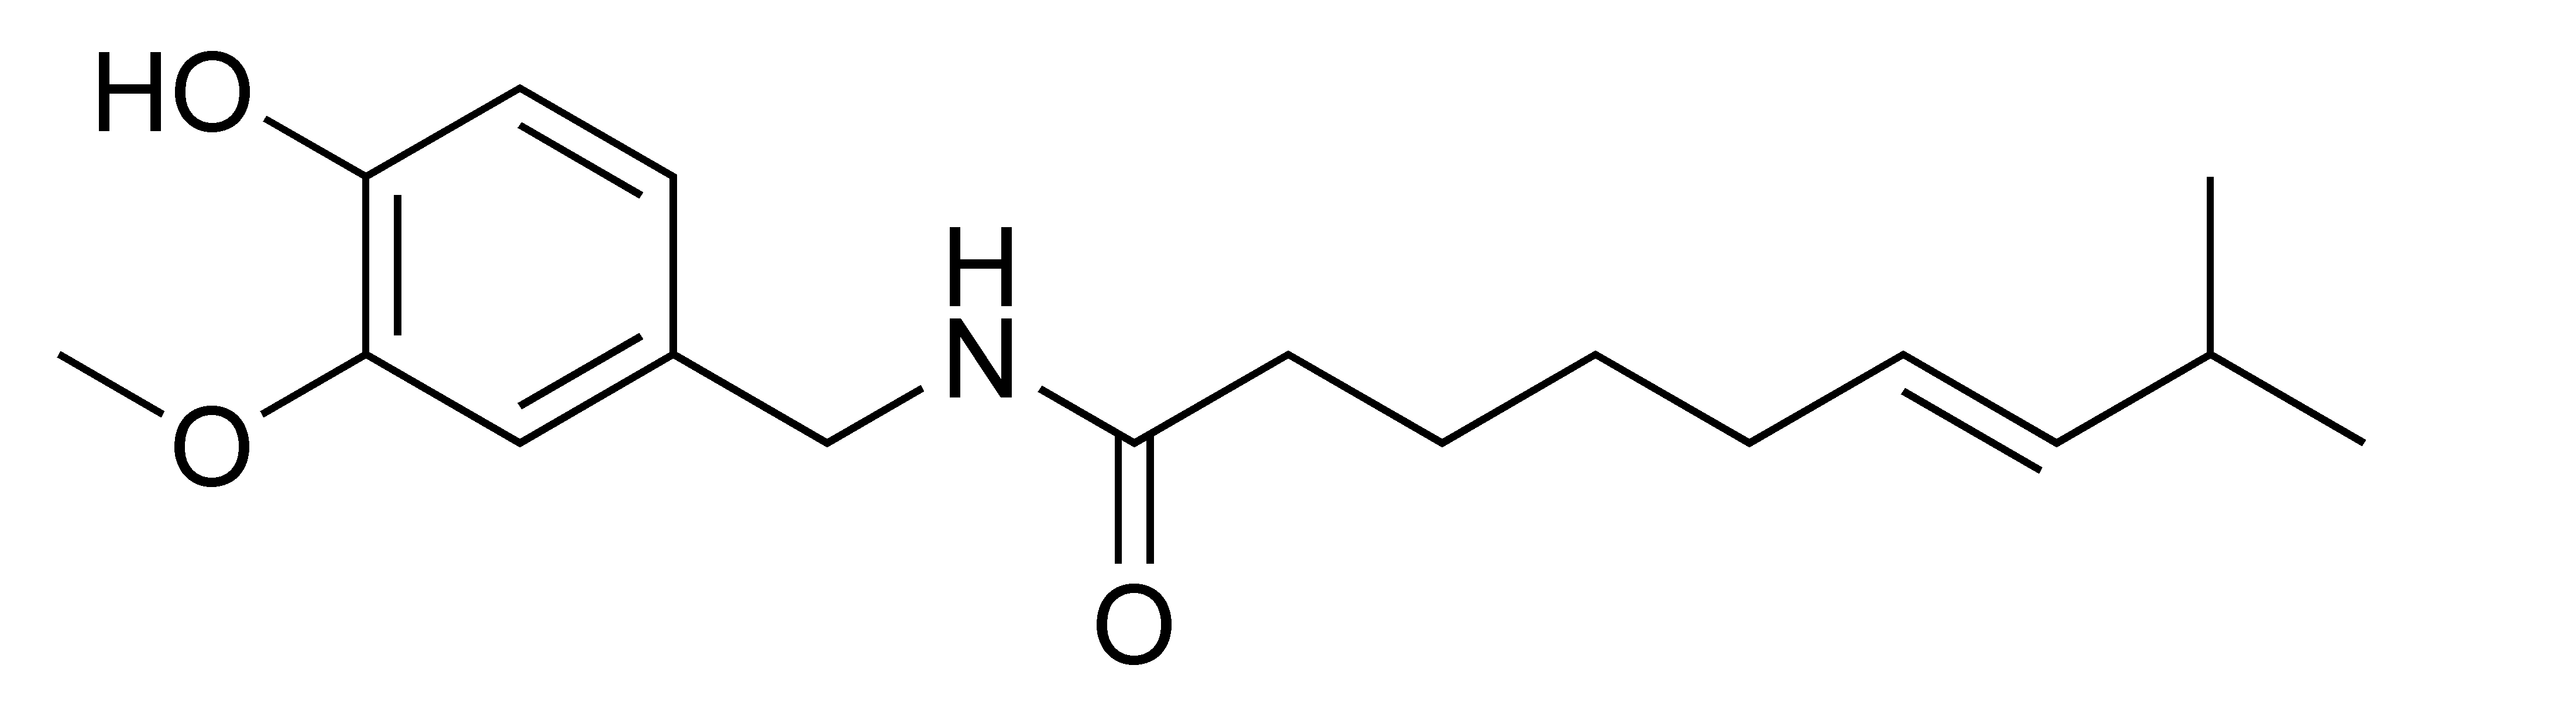
\includegraphics[scale=0.15]{capsaicin}
    \captionof{figure}{Structure of Capsaicin.\cite{lab_man}}
    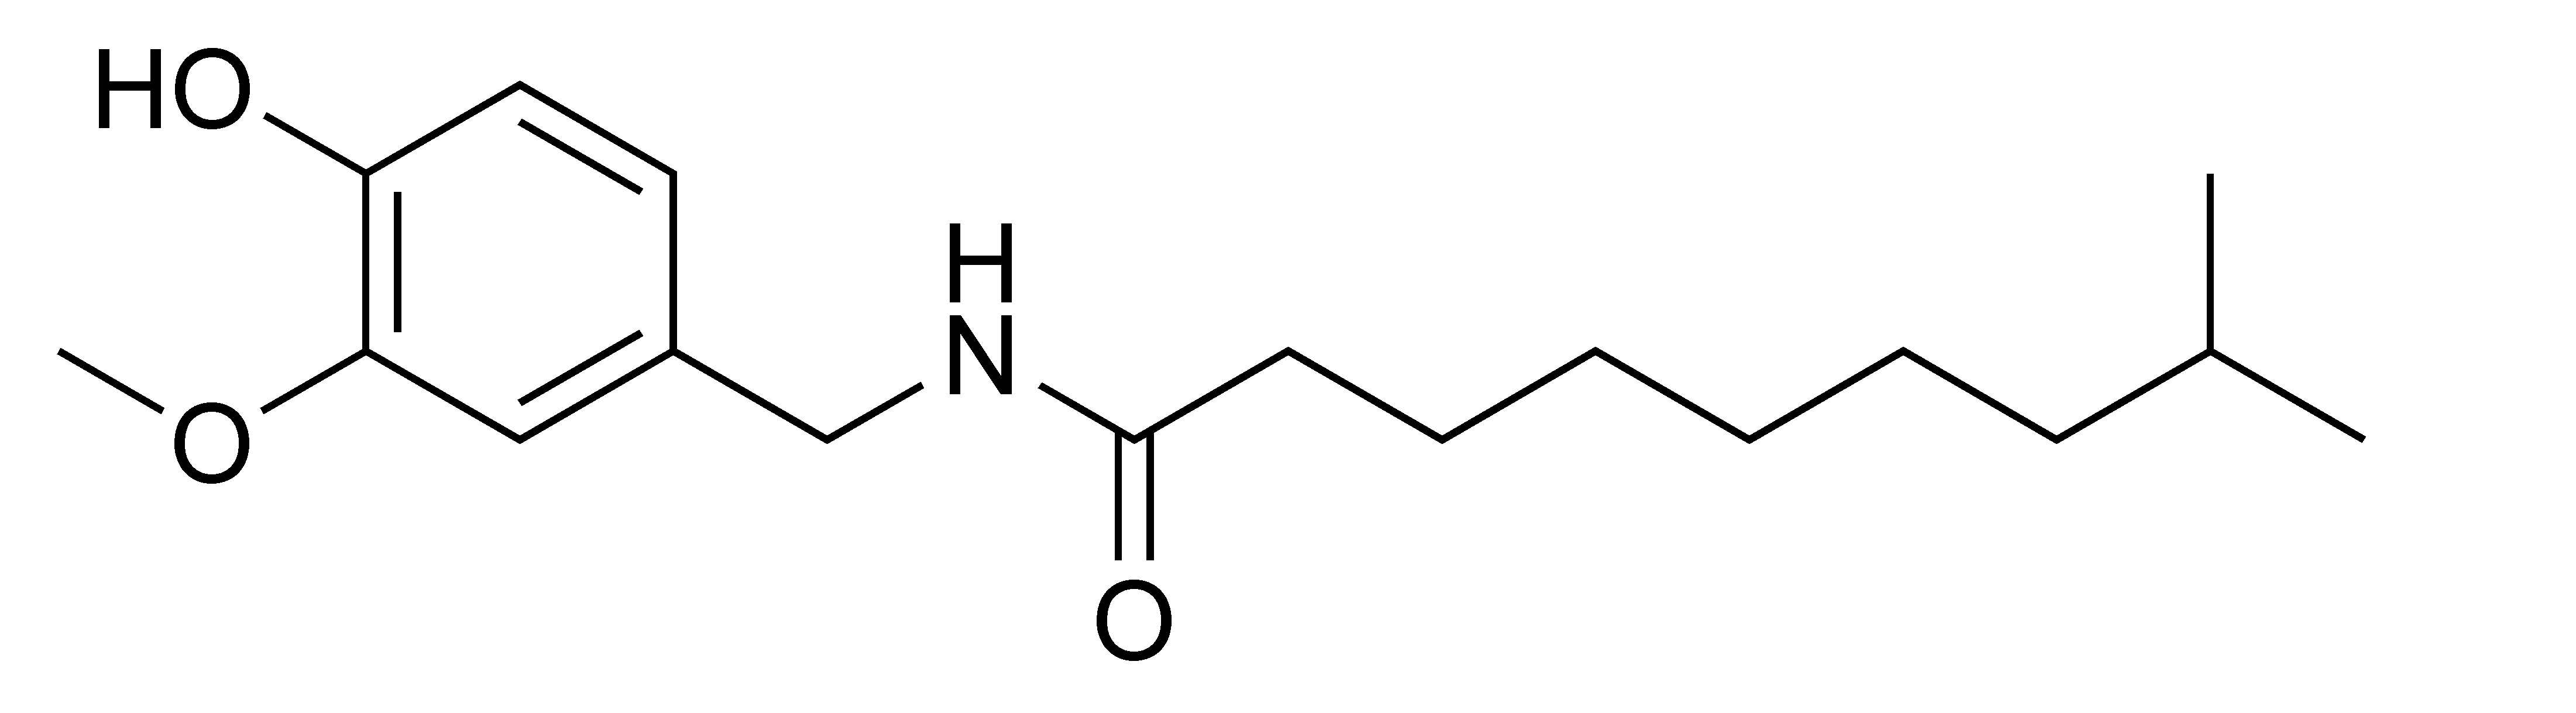
\includegraphics[scale=0.15]{dihydrocapsaicin}
    \captionof{figure}{Structure of Dihydrocapsaicin.\cite{lab_man}}
    \end{center}

\subsection*{HPLC}
High performance liquid chromatography is a type of column chromatography that
    pumps a sample mixture consisting of an analyte in a mobile phase at high
    pressures through a column consisting of chromatographic packing material as
    a stationary phase. 

    Sample retention times vary depending on the interactions of the analyte
    with the stationary phase, the molecules being analyzed, and the solvent(s)
    used. These differences in affinity of the analytes with the mobile and
    stationary phases results in a separation of analytes in the sample mixture
    as it passes through the column that can be quantitatively analyzed upon
    elution with a detector coupled to a data acquisition system.  Analytes with
    the least amount of interaction with the stationary phase or with the most
    amount of interaction with the mobile phase will elute faster.\cite{linde}
    Figure 3 provides a diagram of an HPLC instrument.
    \begin{center}
        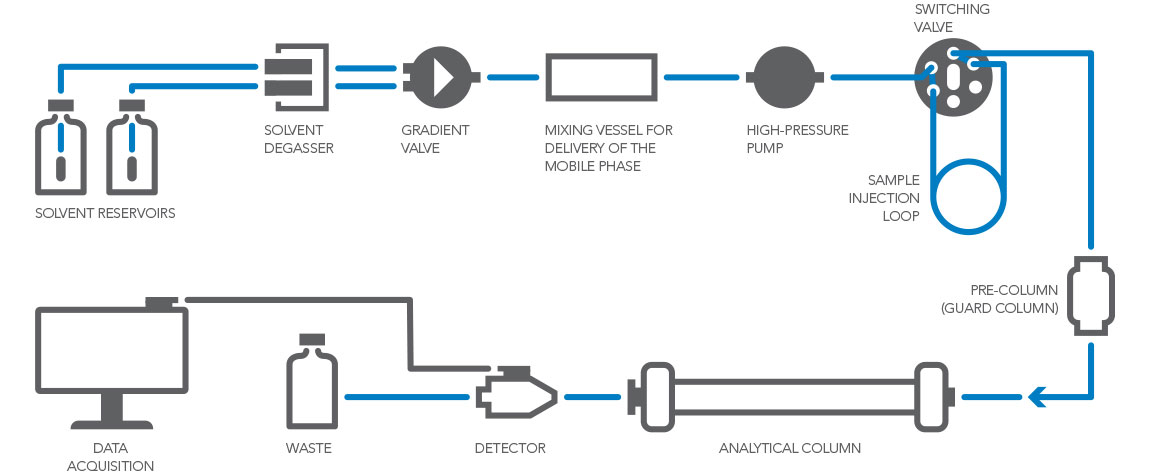
\includegraphics[scale=0.18]{hplc.png} 
        \captionof{figure}{Diagram of an HPLC instrument.\cite{hplc}}
    \end{center}

    Upon analysis of the eluents a chromatogram is produced, where the x-axis
    is the retention time of each analyte in the sample. Each peak corresponds
    to an analyte in the sample, where each peak area equates to the amount of
    analyte detected in the sample.
    Figure 4 shows a chromatogram produced for the unknown sample being analyzed
    in this experiment.
    \begin{center}
        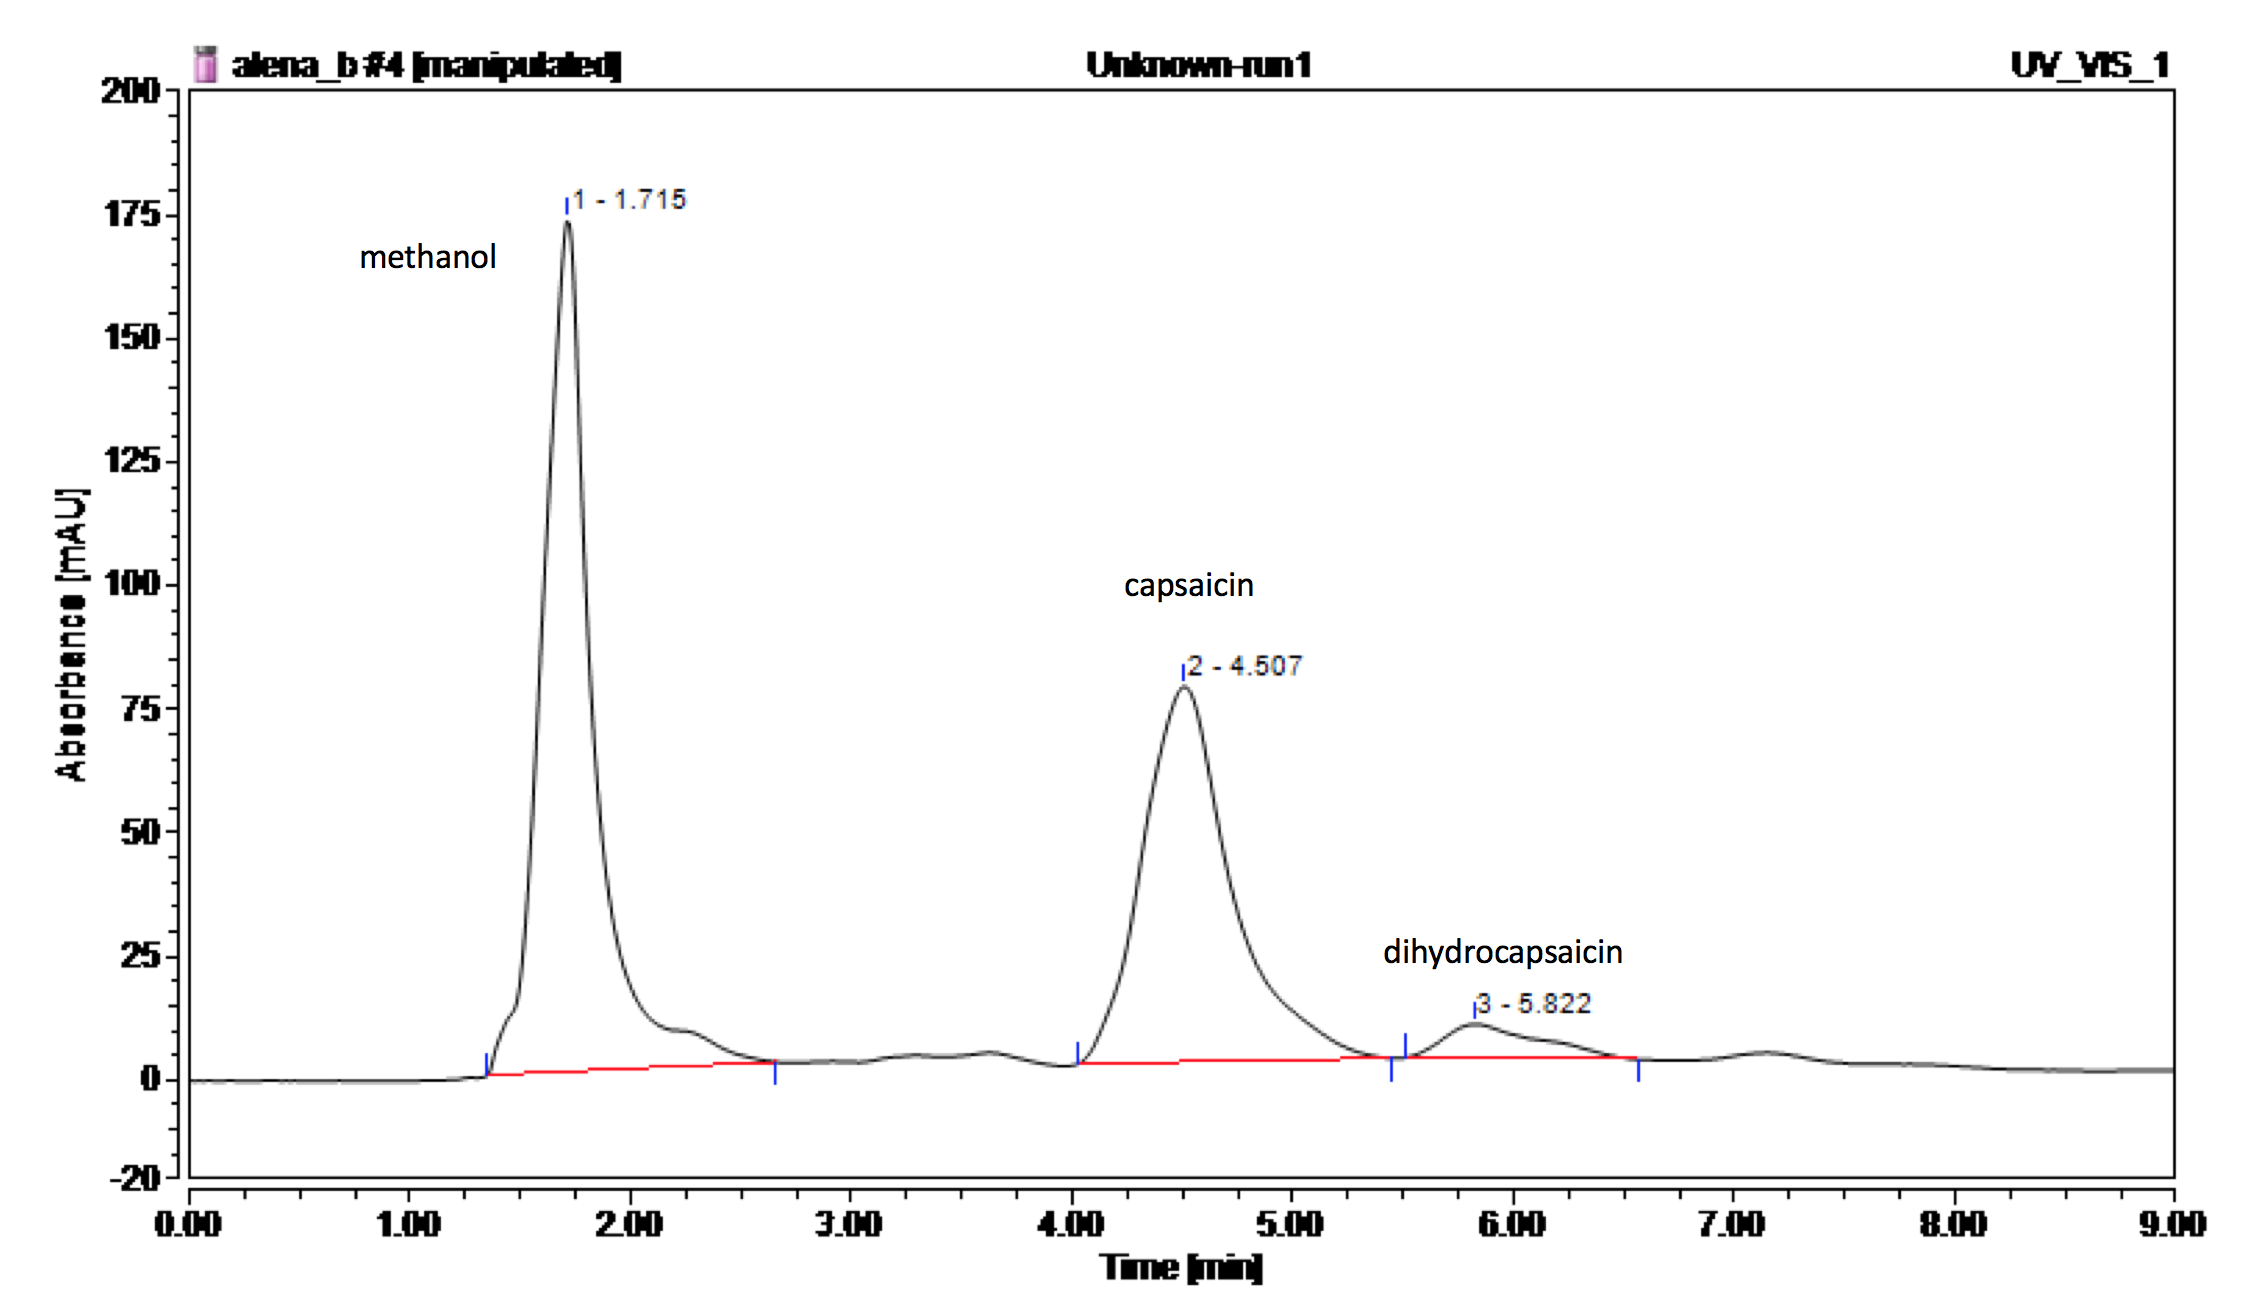
\includegraphics[scale=0.2]{unknown1}
        \captionof{figure}{Chromatogram of Unknown sample.}
    \end{center}

    In a normal-phase HPLC, the stationary phase is polar while the mobile phase
    is non-polar. Silica is often used for the stationary phase. It is also
    typical for normal-phase chromatography to use an organic mobile phase, such
    as hexane.  
    In a reverse-phase HPLC, the stationary phase is non-polar while
    the mobile phase is polar. A C$_{18}$-bonded silica is often used
    for the stationary phase.  Most protocols use an aqueous blend of water with
    a miscible, polar organic solvent, such as acetonitrile or methanol. 
    Due to it's reproducibility and broad
    applicability, reversed-phase chromatography is the preferred method for
    almost 75\% of HPLC methods. \cite{waters}

    There are two types of mobile phase elutions: isocratic and gradient. Under
    isocratic conditions, the mobile phase composition remains constant. Under
    gradient conditions, the solvent strength of the mobile phase is varied
    with time during the chromatographic run. This variation influences the
    retention times of analytes, and allows for the separation to be accelerated
    or decelerated, affecting the end resolution of the produced chromatogram.

    Advantages of HPLC include the ability to quantitate all components of a
    sample mixture. The use of a UV detector also results in very precise retention
    times and peak areas. HPLC also provides for reproducible and
    high-sensitivity assays of trace analytes. 
    The unlimited number of combinations of columns, mobile phases, and
    controlling parameters makes HPLC a complex analytical technique, but gives
    endless possibilities for the quantitation of specific or all components in
    many sample types.
    Disadvantages include less separation efficiency than capillary gas
    chromatography. HPLC can also be very expensive, and has only a moderate
    throughput. \cite{dong}

\subsection*{Solid Phase Extraction}
Solid-phase extraction (SPE), otherwise known as liquid-solid phase extraction,
    is a sample preparation process where compounds that are suspended or dissolved
    in a liquid mixture are separated from other compounds in the mixture by their
    chemical and physical properties. SPE uses the affinity of dissolved or
    suspended analytes in a liquid mobile phase for a solid stationary phase through
    which the sample is passed through to separate the analytes from other undesired
    components in the sample mixture.  The solid stationary phase is usually
    contained in a cartridge type device. The liquid sample is then passed through
    the cartridge, where it can be effectively separated.
    Figure 5 shows a sample, which appears black, being separated using SPE,
    resulting in the individual dye compounds.
    \begin{center}
        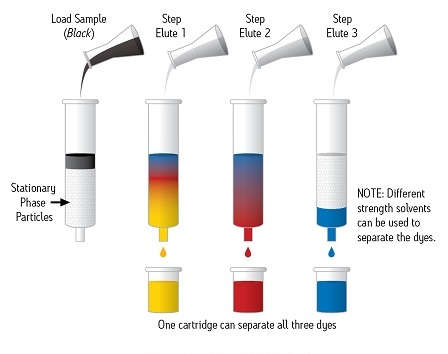
\includegraphics[scale=0.4]{spe}
        \captionof{figure}{Solid-phase extraction of a sample into its individual
        dye compounds.\cite{linde}}
    \end{center}

\subsection*{Scoville Method}
The Scoville scale is a subjective measurement of the heat of chili peppers,
    dependent on the capsaicin sensitivity of testers. Unlike methods such as HPLC,
    the Scoville scale is not a precise or accurate method to measure the capsaicinoid
    concentrations of peppers. Disadvantages of the Scoville Organoleptic Test include its
    imprecision due to its dependency on the test taster's palate and number of
    heat receptors in the mouth, as these factors can vary greatly among people. Another
    disadvantage includes the sensory fatigue of the test taster, where the palate
    becomes desensitised to capsaicins after tasting a few sample within a short
    period of time.

\section*{Experimental}
\subsection*{Instrumental Parameters}

A Dionex UltiMate\textsuperscript{TM} 3000 UHPLC system equipped with an
    Acclaim\textsuperscript{\textregistered} 120, 15 cm C$_{18}$ hydrocarbon reverse
    phase column, a 20 μL injection loop, and a variable wavelength UV-Vis
    absorption detector was used in this experiment.
    The column consisted of a particle size of 3μm and an average pore diameter of
    120 \AA. \cite{dionex}

    A mobile phase mixture of 25\% H$_2$O and 75\% methanol was used with a flow
    rate of 0.5 mL/min and max back pressure of 3447 psi.

    All mobile phase solvents were degassed and filtered to minimize the amount of
    particulate traveling through the column. 
    A C$_{18}$ guard column was also used.

    In this experiment, an UltiMate\textsuperscript{TM} 3000 Variable Wavelength UV-Vis
    Absorption Detector set at 280 nm was used, with a data collection rate of 100.0
    Hz.

\subsection*{Sample Preparation}
A standard solution diluted with methanol from a 65\% capsaicin / 35\%
    dihydrocapsaicin mixture was prepared and diluted into three separate 10 mL
    standard solutions using 1-, 2-, and 5-mL aliquots. Each standard solution was
    then filtered through a glass filtering syringe, and 50μL of each filtrate was
    then injected into the HPLC for analysis.

    A mass of 8.7797 g of the hot sauce sample was weight out, pulverized with a
    mortar and pestle, filtered through filter paper, and diluted to 25 mL with acetonitrile.
    A volume of 2 mL of the filtered unknown sample was then transferred into two 10
    mL volumetric flasks. A volume of 1 mL of the capsaicinoid stock solution was
    added to one of the flasks as the spiked unknown. Both flasks were then diluted
    to 10 mL with high purity water.

    Two SPE cartridges were conditioned by flowing 6 mL amounts of methanol,
    acetonitrile, and high purity water through the cartridge. Each unknown sample
    was then passed through a conditioned SPE cartridge. The retained compounds
    were then eluted using 4 mL of methanol and 1 mL of a methanol with 1\% acetic
    acid solution.

    After extraction, both unknown samples were filtered using a glass filtering
    syringe. Each unknown sample was then injected into HPLC for analysis.
    The unknown and spiked unknown samples were run three times each.


\section*{Results}

Figures 6 and 7 shows the constructed calibration curves for capsaicin and
dihydrocapsaicin from the standard solutions.
\begin{center}
    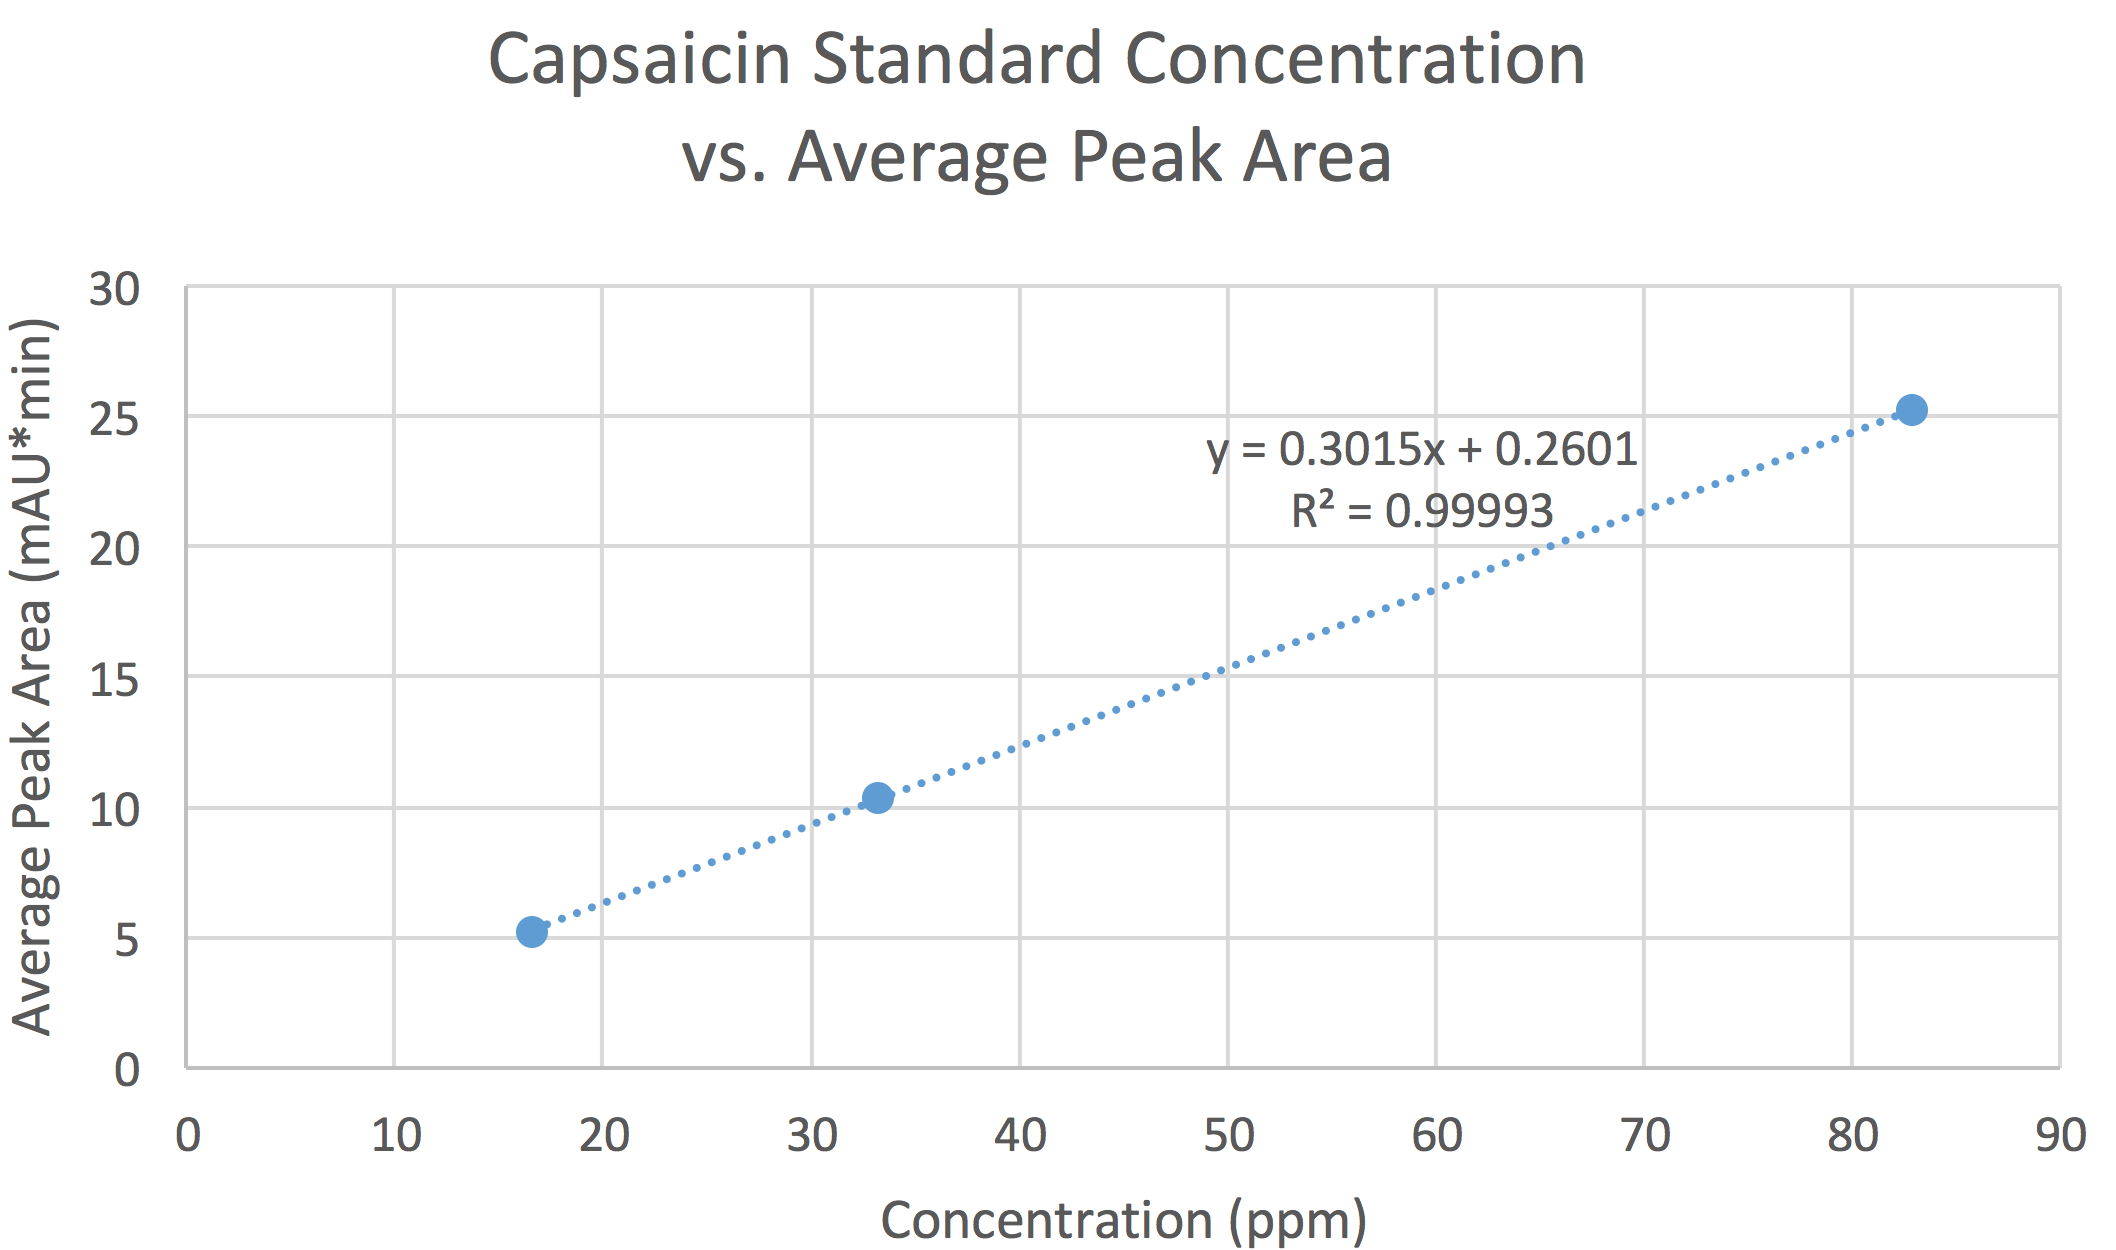
\includegraphics[scale=0.2]{calibration_capsaicin}
    \captionof{figure}{Calibration curve for capsaicin generated from standard solutions.}
    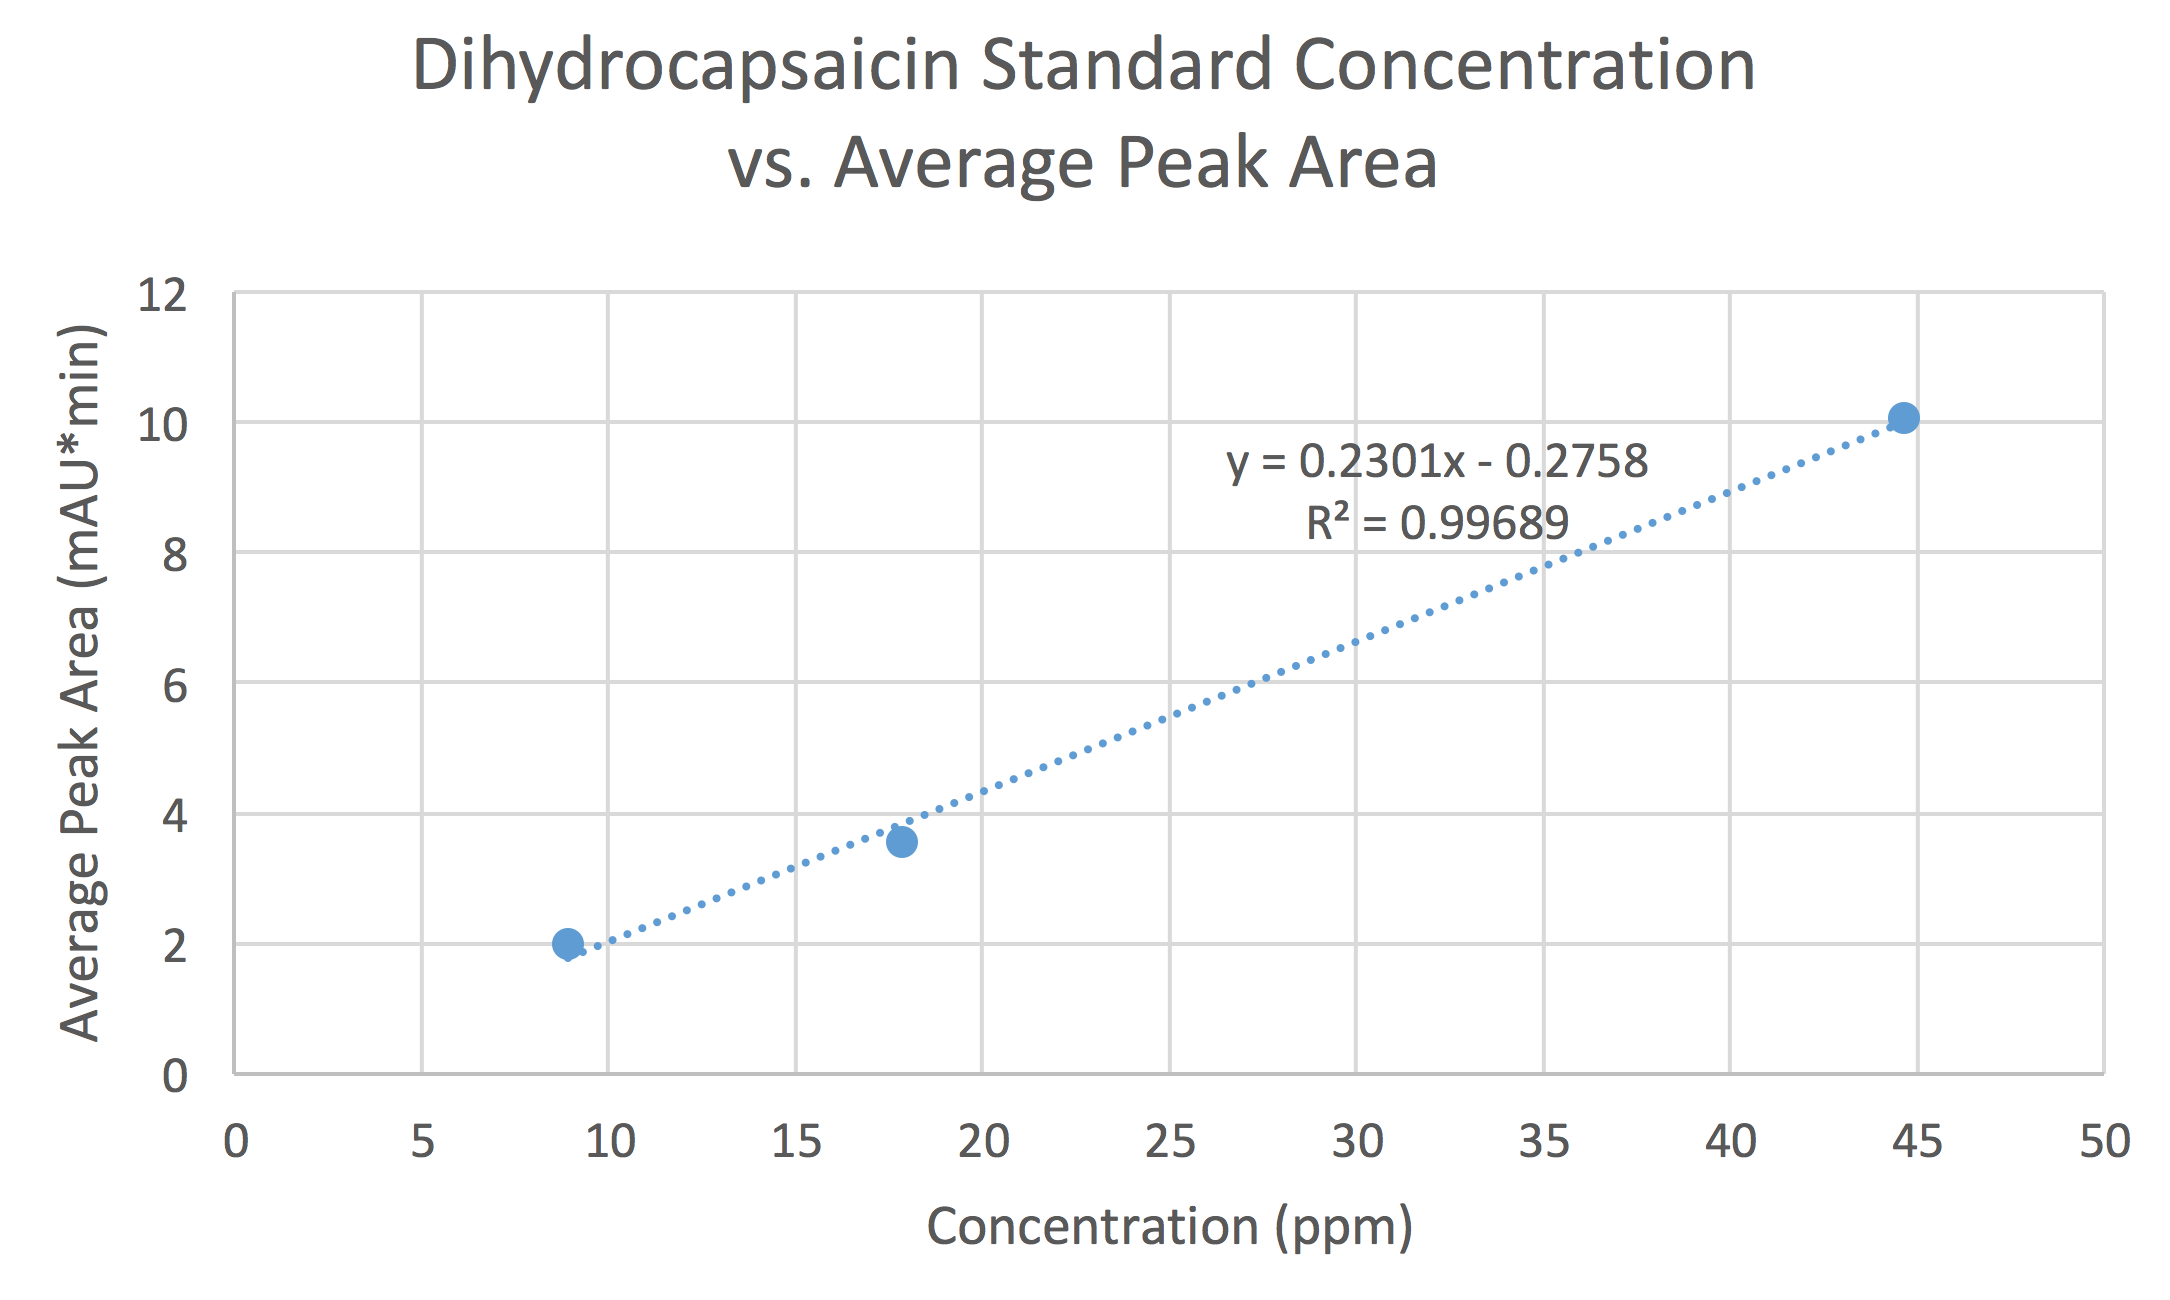
\includegraphics[scale=0.2]{calibration_dihydrocapsaicin}
    \captionof{figure}{Calibration curve for dihydrocapsaicin generated from standard solutions.}
\end{center}

Table 1 lists the capsaicinoid concentrations for the unknown and spiked
unknown solutions as determined from the calibration curves. 
\begin{center}
	\captionof{table}{Capsaicinoid concentrations as determined from calibration curves.}
    \resizebox{0.45\textwidth}{!}{\begin{tabular}{lrrr}
        & \multicolumn{1}{l}{Capsaicin} & \multicolumn{1}{l}{Dihydrocapsaicin} &
        \multicolumn{1}{l}{Total}\\
	\hline
        Unknown (ppm) & 115.0 $\pm$ 0.6 & 14.8 $\pm$ 1.06 & 129.8 $\pm$ 1.66 \\
        Spiked unknown (ppm) & 158.3 $\pm$ 0.7 & 33.02 $\pm$ 0.28& 191.32 $\pm$
        0.98 \\
    \end{tabular}}
\end{center}

Table 2 lists the heat ratings for capsaicin and dihydrocapsaicin found in the
unknown hot sauce sample.
\begin{center}
    \captionof{table}{Heat ratings for capsaicinoids found in unknown hot sauce sample.}
    \resizebox{0.4\textwidth}{!}{\begin{tabular}{lr}
	Capsaicinoid & Heat Rating (Scoville Units) \\
	\hline
    Capsaicin & 26404 $\pm$ 138\\
    Dihydrocapsaicin & 3381 $\pm$ 243\\
	Total & 29785 $\pm$ 381\\
    \end{tabular}}
\end{center}

The values found for the heat rating of the hot sauce sample are within range
and consistent with those listed for Tabasco\textsuperscript{\textregistered}
(30,000 - 50,000 Scoville Units), as gathered from a range of references.
Therefore, it is concluded that the obtained values are precise and accurate.

\section*{Discussion}
The results obtained in this experiment are within expected values, however,
precision may be improved with the inclusion of more sample runs. Methods to
improve experiment run times may include increasing the temperature and flow
rate of the mobile phase while decreasing pore size.
While many capsaicinoids are present in peppers, it is assumed that the majority
of the heat accounted for in chili peppers comes from capsaicin and
dihydrocapsaicin. Therefore, only these two capsaicinoids were analyzed in this
experiment.

[1] Reversed-phase SPE retains most molecules with hydrophobic characteristics.
This method is usually used to extract organic analytes from aqueous samples by
disrupting reversed-phase interactions of the analytes with the sorbent
functional groups using solvent mextures of adequate non-polar character, such
as methanol, acetonitrile, or dichloromethane.  Prior to loading the sample
matrix, the SPE cartridge is conditined to activate the bonded phases to ensure
that there is consistent interactions between the sorbent functional groups and
the analyte. A wash step is then conducted to elute interferences without
eluting the analytes. Finally, the retained compounds of interest are extracted
by disrupting the hydrophobic interactions between the analyte and the sorbent
functional groups with a solvent mixture of sufficient non-polar character.
Figure 8 illustrates the retention mechanism of a reversed-phase SPE cartridge.
\begin{center}
    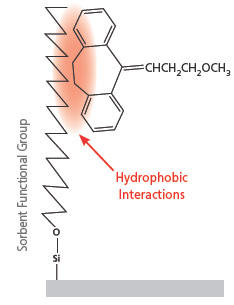
\includegraphics[scale=0.4]{spe_cartridge}
    \captionof{figure}{Retention mechanism of a reversed-phase SPE
    cartridge.\cite{waters}}
\end{center}

[2] A separation of the two capsaicinoids using a reverse phase HPLC column
would would cause capsaicin to elute first, then dihydrocapsaicin. This is
because the double bond found on capsaicin lowers its retention factor for
hydrophobic, non-polar interactions with the stationary phase. The lack of a
double bond on dihydrocapsaicin results in a longer retention time due to its
ability to interact with the non-polar stationary phase on a greater level.

[3a] A spiked sample was used in addition to the unknown sample to allow for the
evaluation of the performance of the detection system. 
[3b] A percent recovery obtained from a spiked sample vs. an unspiked
sample increases the confidence in accuracy and validity of the results by
allowing for the determination of whether a systematic shift in the analytical
signal occurs due to matrix effects.
[3c] For both capsaicinoids analyzed in this experiment, a percent recovery
signal of 100\% was obtained, indicating that the results obtained for the
unknown sample are analytically accurate.

[4a] In this experiment, HPLC was used to quantify and separate the capsaicinoid
content in hot sauce due to the low volatility and trace concentration of the
sample being analyzed.
[4b] Capillary electrophoresis would be a more suitable alternative for
analyzing capsaicinoid content than gas chromatography 
[4c] due to the low volatility of the analytes, low concentration amounts being
used, and ability of the analytes to hold a charge under corrected
circumstances.

[5a] The effects of linear flow rate on the height equivalent of a theoretical
plate in separation can be described by the van Deemter equation. In HPLC with a
packed column, the A term has the largest effect on
the separation efficiency, representing the multiple pathways that a molecule
can take down the separation column. Furthermore, retention factors between the mobile and
stationary phases may also impact the C term, representing the equilibration
time.
[5b] Figure 9 shows a qualitative van Deemter plot for this experiment.
\begin{center}
    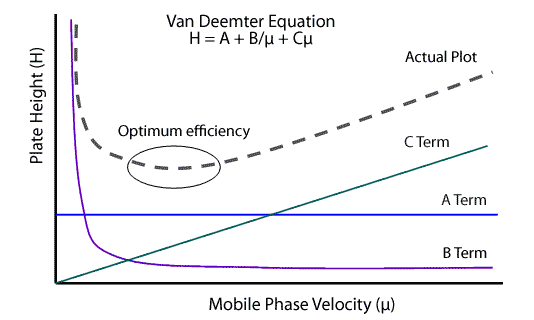
\includegraphics[scale=0.4]{vanDeemter}
    \captionof{figure}{Qualitative van Deemter plot for this
    experiment.\cite{van}}
\end{center}
[5c] Physical parameters that can be adjusted to increase the efficiency of HPLC
separation include increasing pressure and temperature while decreasing column
diameter, decreasing particle size of the stationary phase to increase the A
term, and increasing column length. Adjusting mobile phase compositions may also
increase the retention factor, allowing for higher resolutions of peaks.
[5d] Increasing column length would result in longer retention times and longer
run times. However, this can be mitigated if the column diameter were to be
decreased and the pressure and temperature increased, keeping run times in
reasonable domain. Changing mobile phase compositions, such as using a gradient
composition can be easily accomplished, however changing the particle sizes of a
packed column can get costly.

[6] In a previous experiment, an analysis of a recreational alcohol was carried
out using gas chromatography. This method afforded HETP values of around 0.2 mm.
This is similar to values obtained in this experiment using HPLC. It can be
concluded that both GC and HPLC are equally precise in analytically separating
and determining the componenets of a mixture, given optimal parameters and
conditions.


\subsection*{Literature Review}
A another study that uses HPLC includes the "Determination of
sec-O-glucosylhamaudol in rat plasma by gradient elution liquid
chromatography–mass spectrometry".\cite{rat}
In this article, chromatographic separation was achieved on a Zorbax SB-C18
column.
A gradient elution program was conducted for chromatographic separation with
mobile phase A (0.1\% formic acid), and mobile phase B (acetonitrile) as follows:
0–4.0 min (10–80\% B), 4.0–7.0 min (80–80\% B), 7.0–8.0 min (80–10\% B), 8.0–13.0
min (10–10\% B).
The flow rate was 0.4 mL/min.
Calibration standards were prepared by spiking blank rat plasma with appropriate
amounts of the workign solutions. Calibration plots were constructed in the
range of 50-8000 ng/mL for sec-O-glucosylhamaudol in rat plasma.
Quality control sampels were also prepared in the same way as the calibration
standards.
The retention time of sec-O-glucosylhamaudol under experimental conditions was
found to be 5.9 min.

\section*{Conclusion}
The total heat rating for the Tabasco\textsuperscript{\textregistered} hot sauce
used in this experiment was found to be 29785 $\pm$ 381 Scoville Units. As
compared to Typical Scoville Ratings for common peppers\cite{lab_man}, it can be determined
that the hot sauce sample may contain any or all of the following peppers:
Pequin, Cayenne, Tabasco, Rocoto, and Aji Rojo.
The results found in this experiment are consistent with those in literature
\cite{lab_man},
and are concluded to be reproducible, precise, and accurate. 
Sources of error may include random error on the part of the preparation of
samples, as multiple people were involved in the process. Systematic error in
the handling of the HPLC instrument and injection of sample runs may have also
been a factor. These sources of error may cause a loss of precision in
determining retention times and peak areas of produced chromatograms, leading to
incorrect analysis of capsaicinoid concentration amounts.


\bibliography{HPLC.bib}

}
\end{multicols}



\newpage
\section*{Appendix}
\begin{enumerate}
    \item Chromatograms of standard, sample, and spiked sample runs.
    \item Tabular raw data.
    \item Sample calculations of determining heat rating of capsaicin in
        unknown sample.
    \item Laboratory notebook copies.
\end{enumerate}

\newpage
\begin{center}

    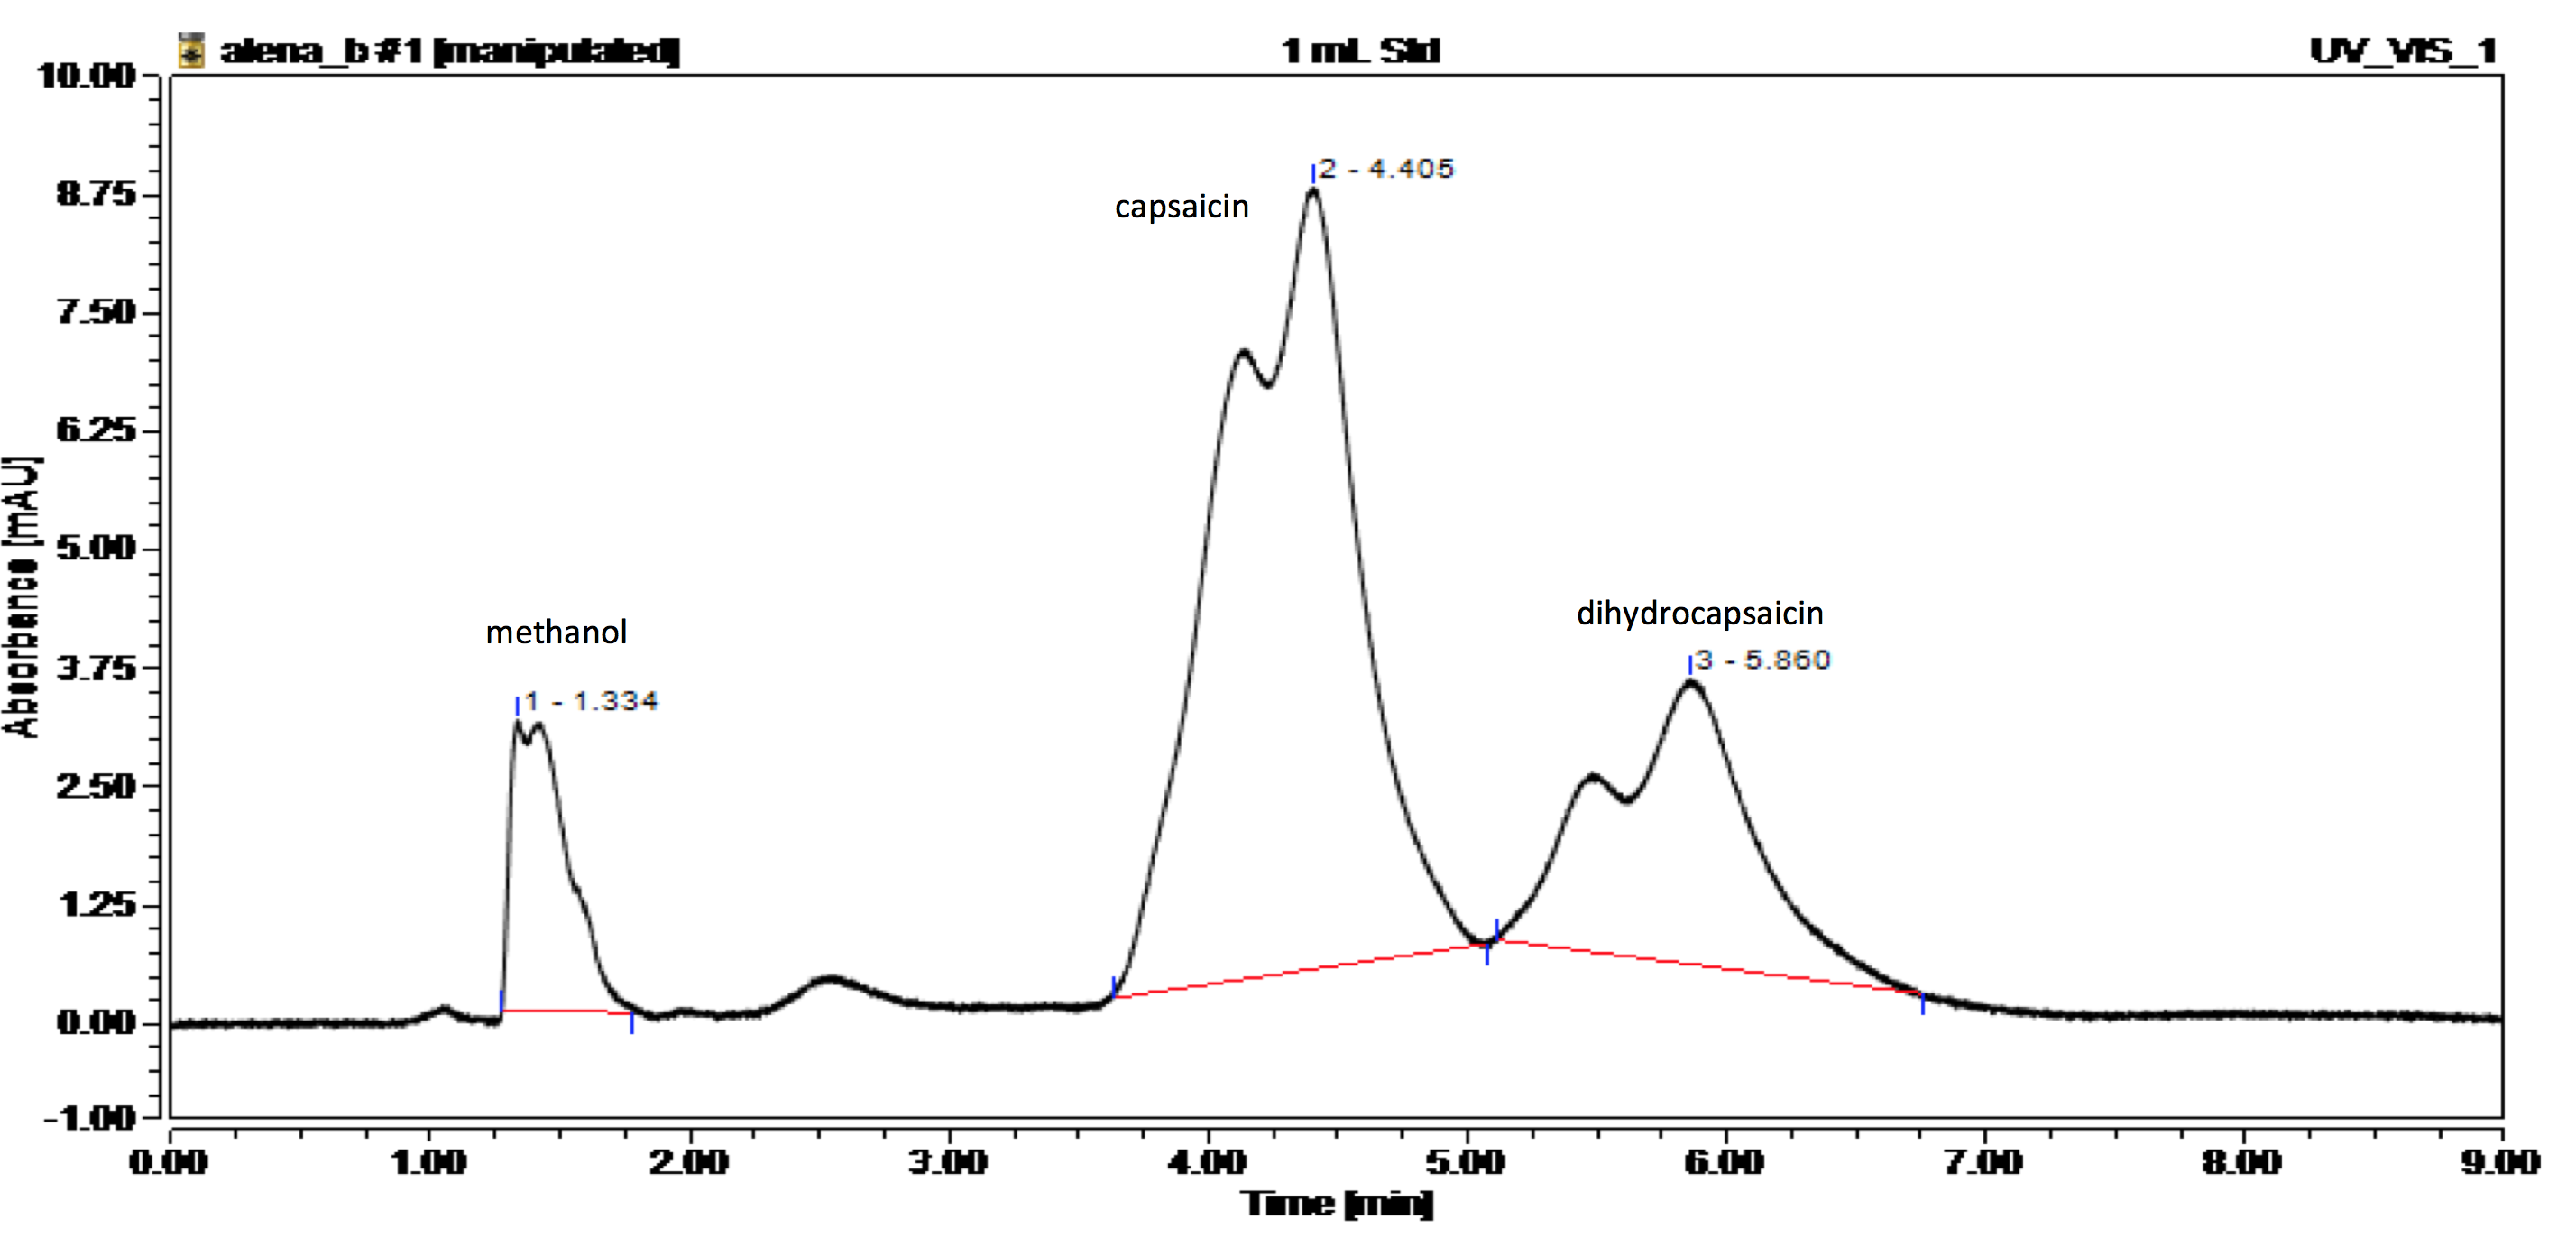
\includegraphics[scale=0.25]{1mL}
    \captionof{figure}{Chromatogram of 1 mL standard solution.}

\vspace{5cm}
    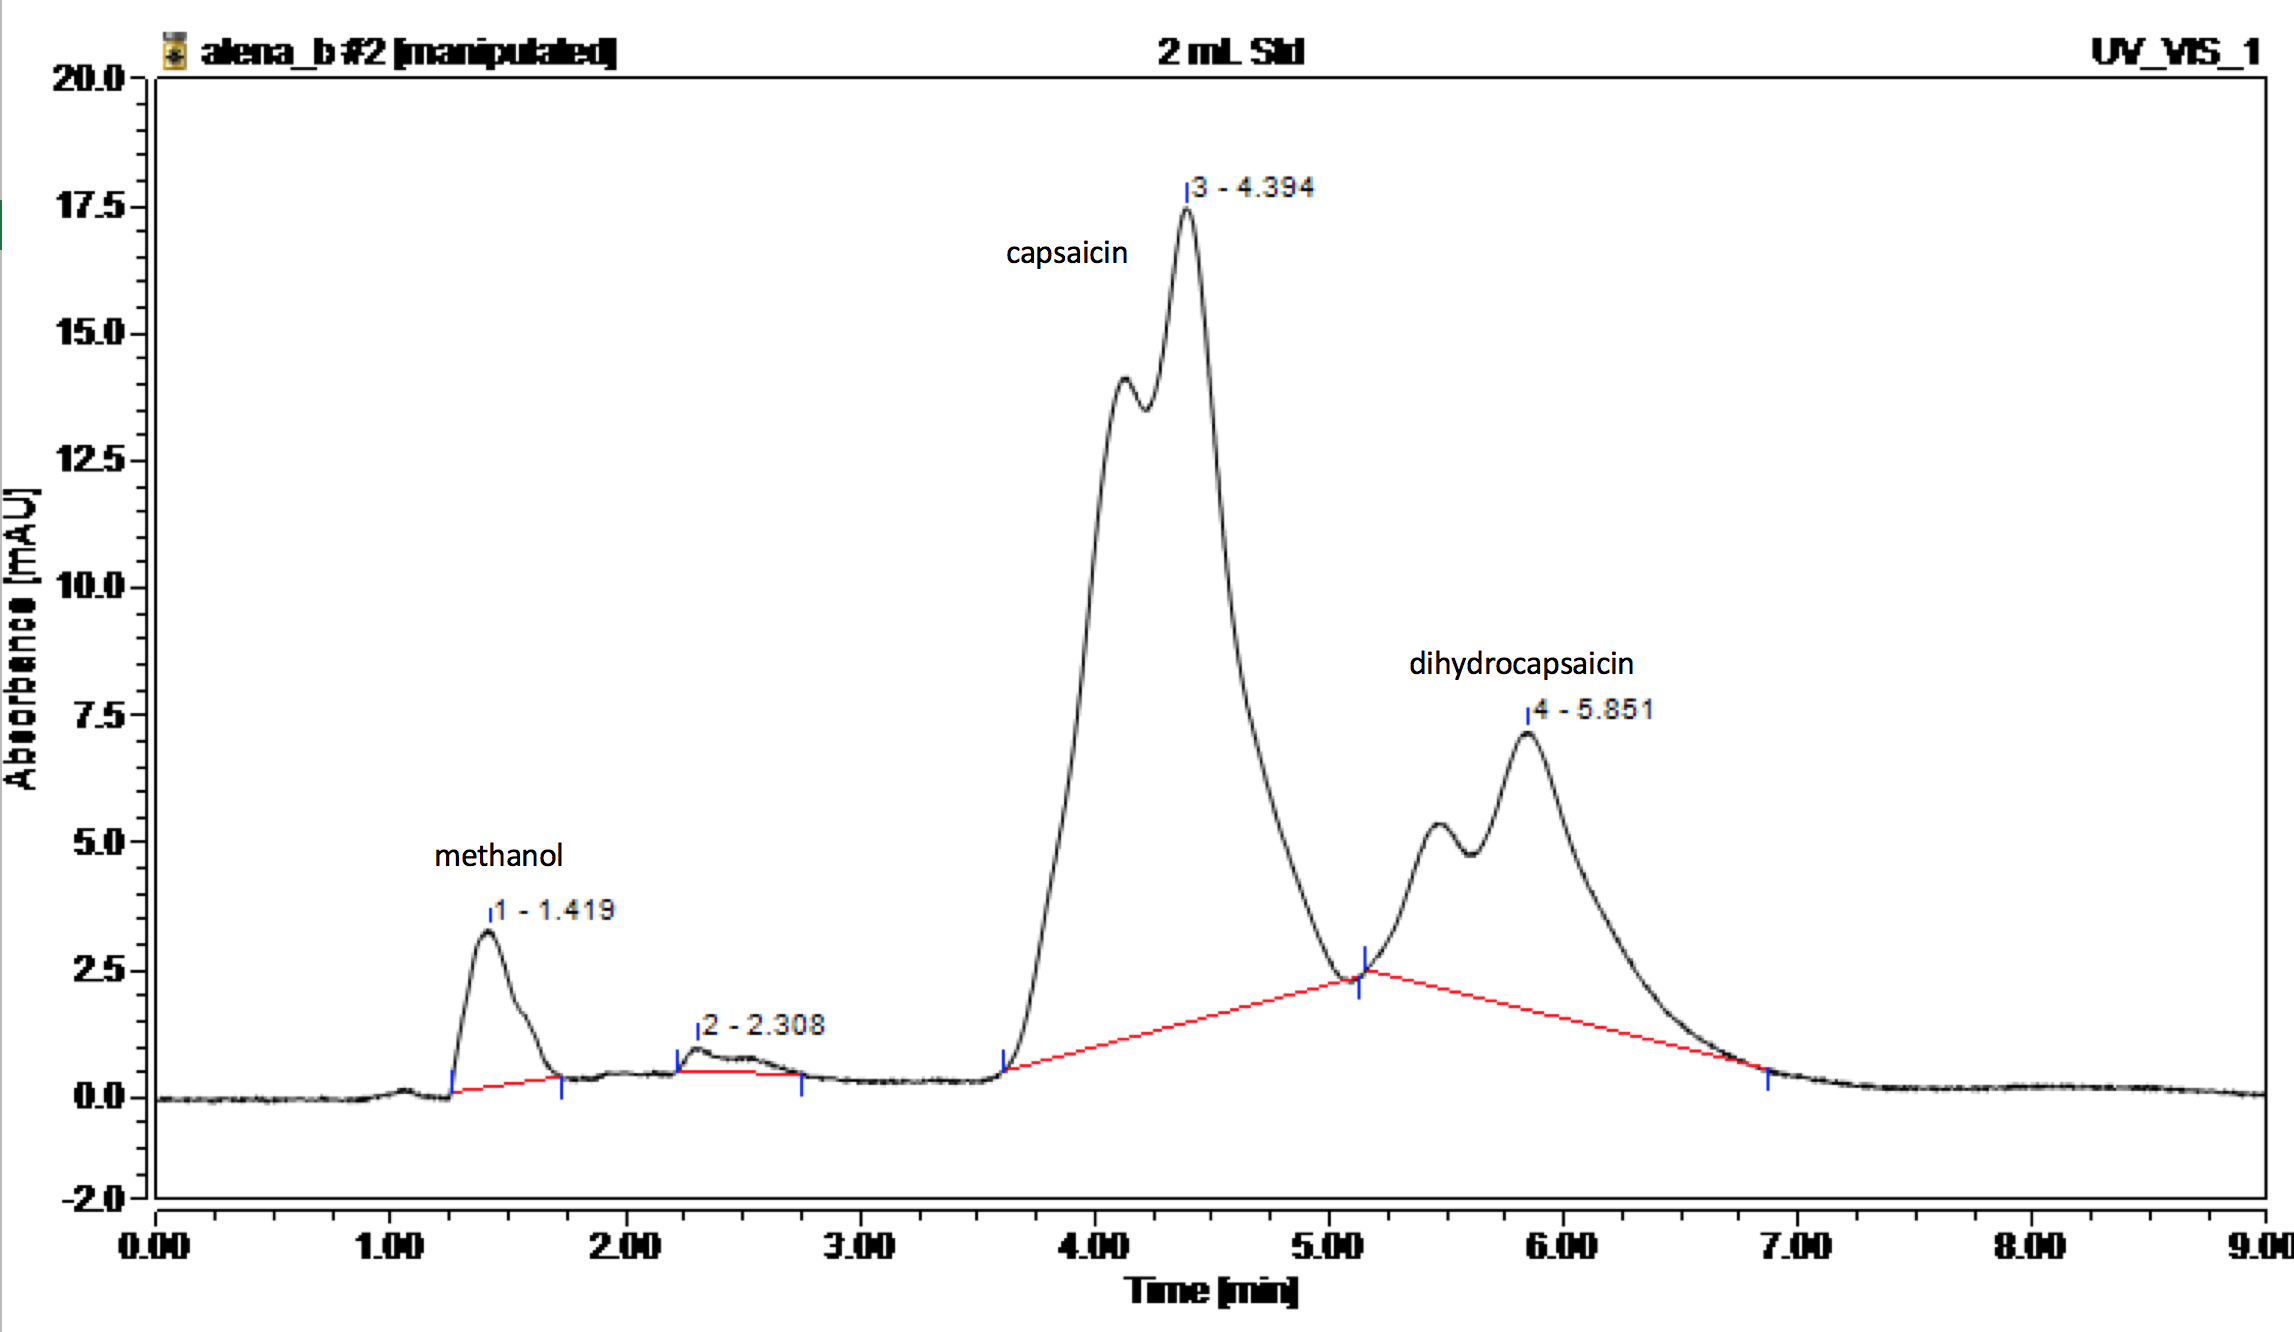
\includegraphics[scale=0.3]{2mL}
    \captionof{figure}{Chromatogram of 2 mL standard solution.}

\vspace{5cm}
    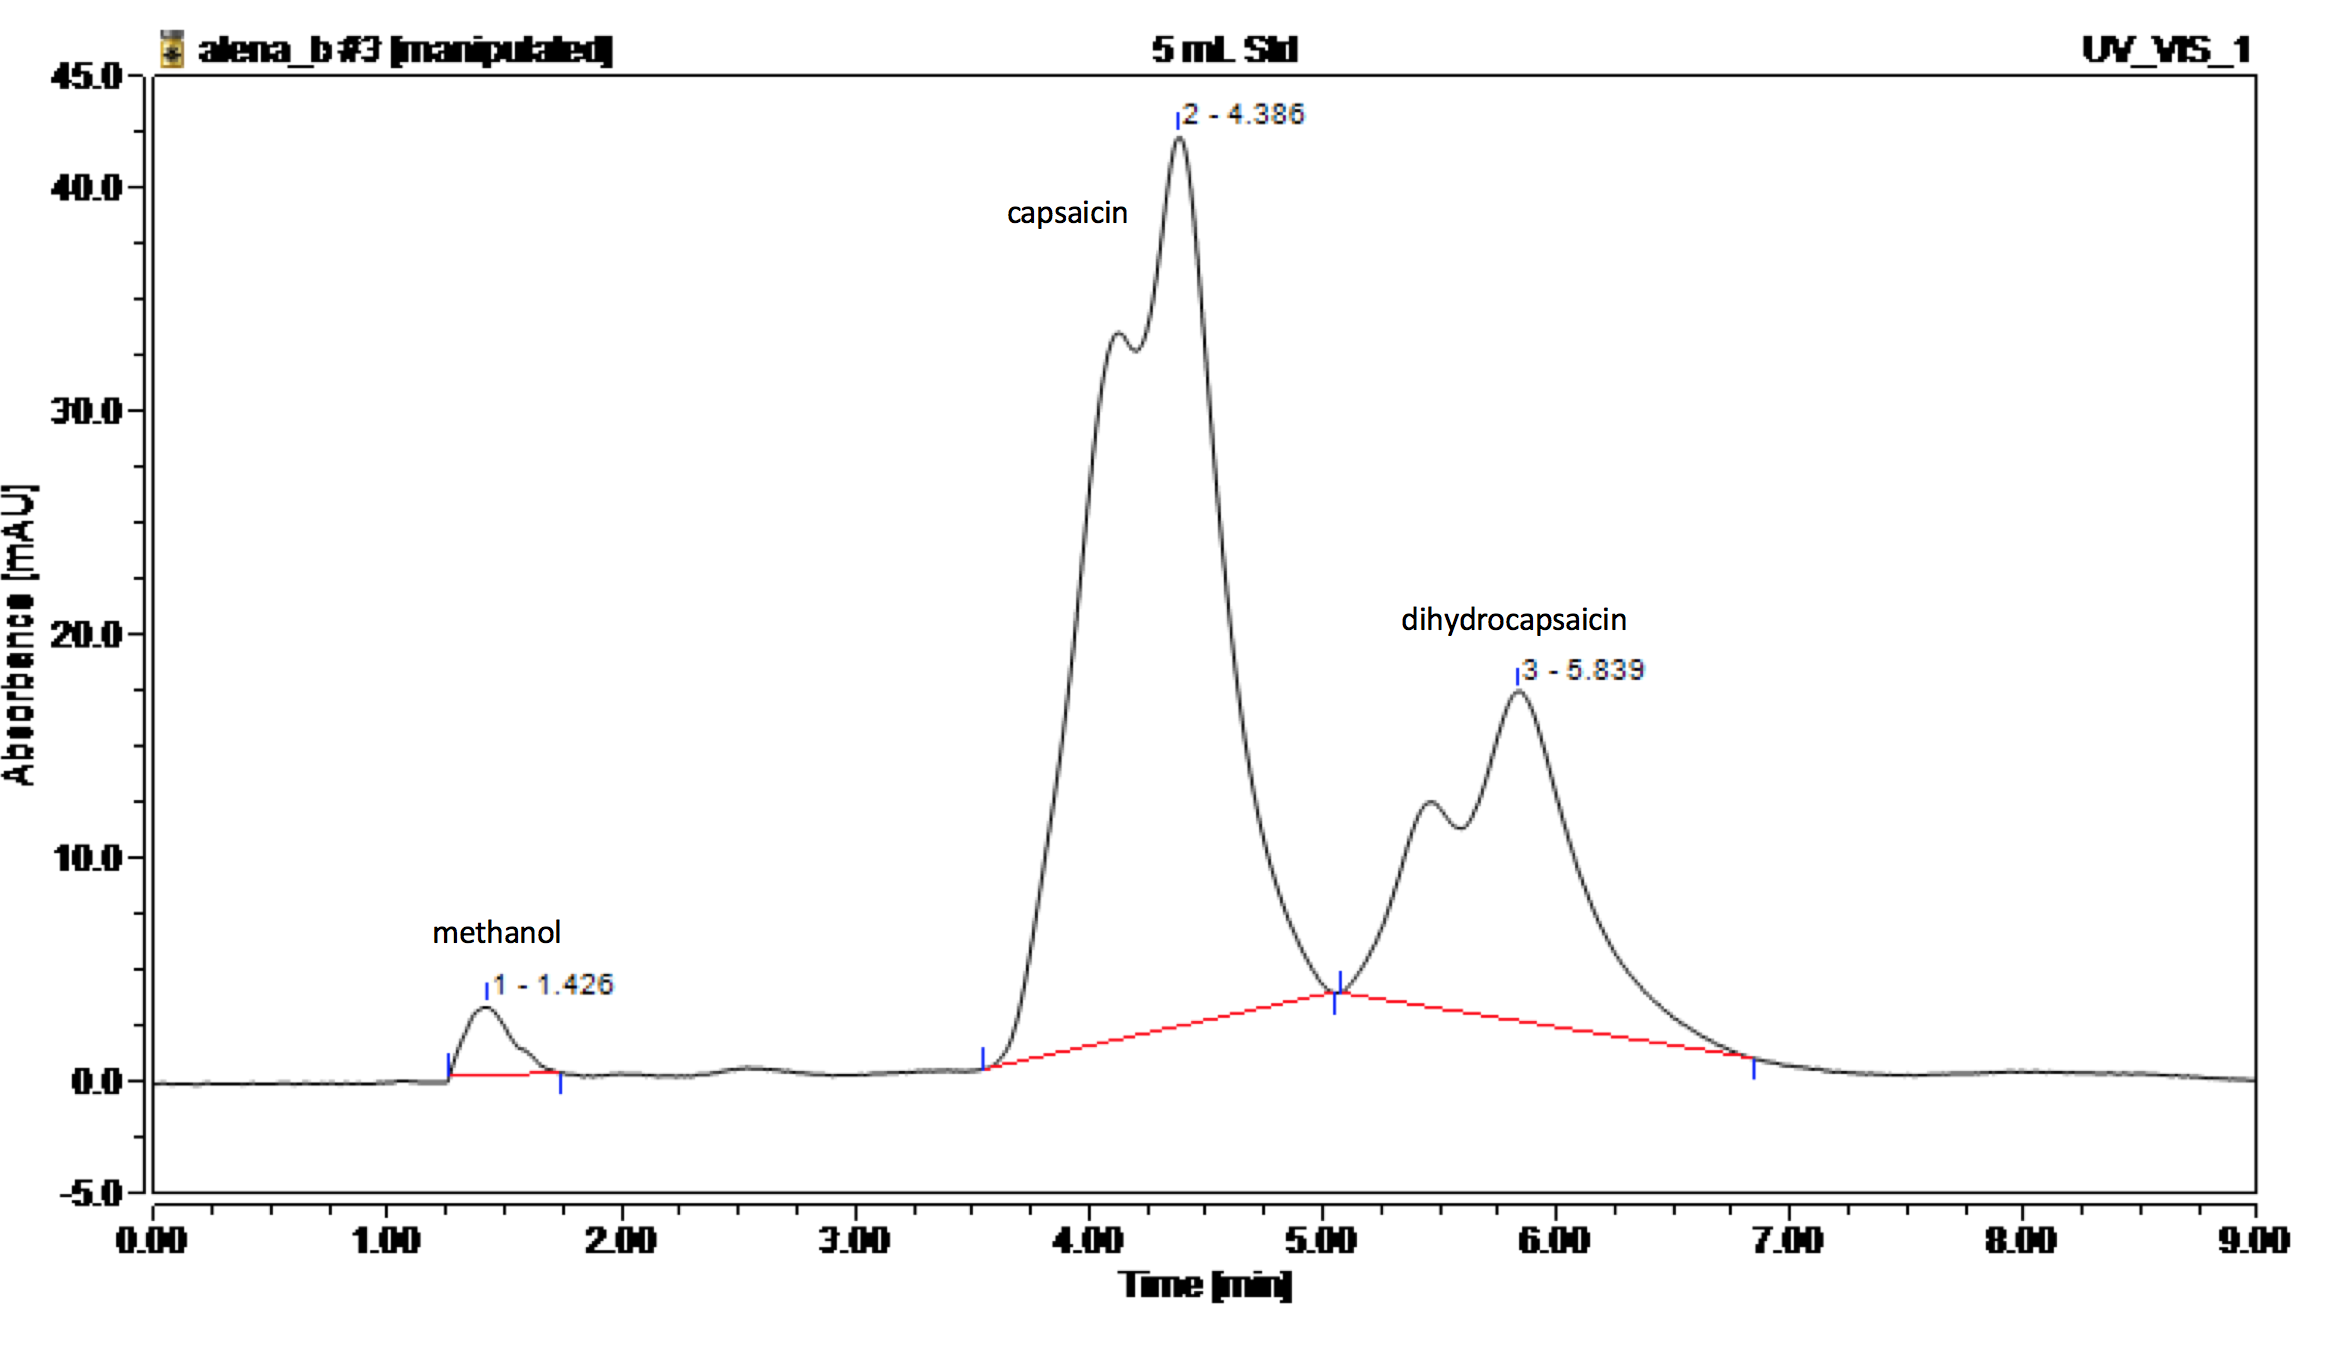
\includegraphics[scale=0.3]{5mL}
    \captionof{figure}{Chromatogram of 5 mL standard solution.}

\vspace{5cm}
    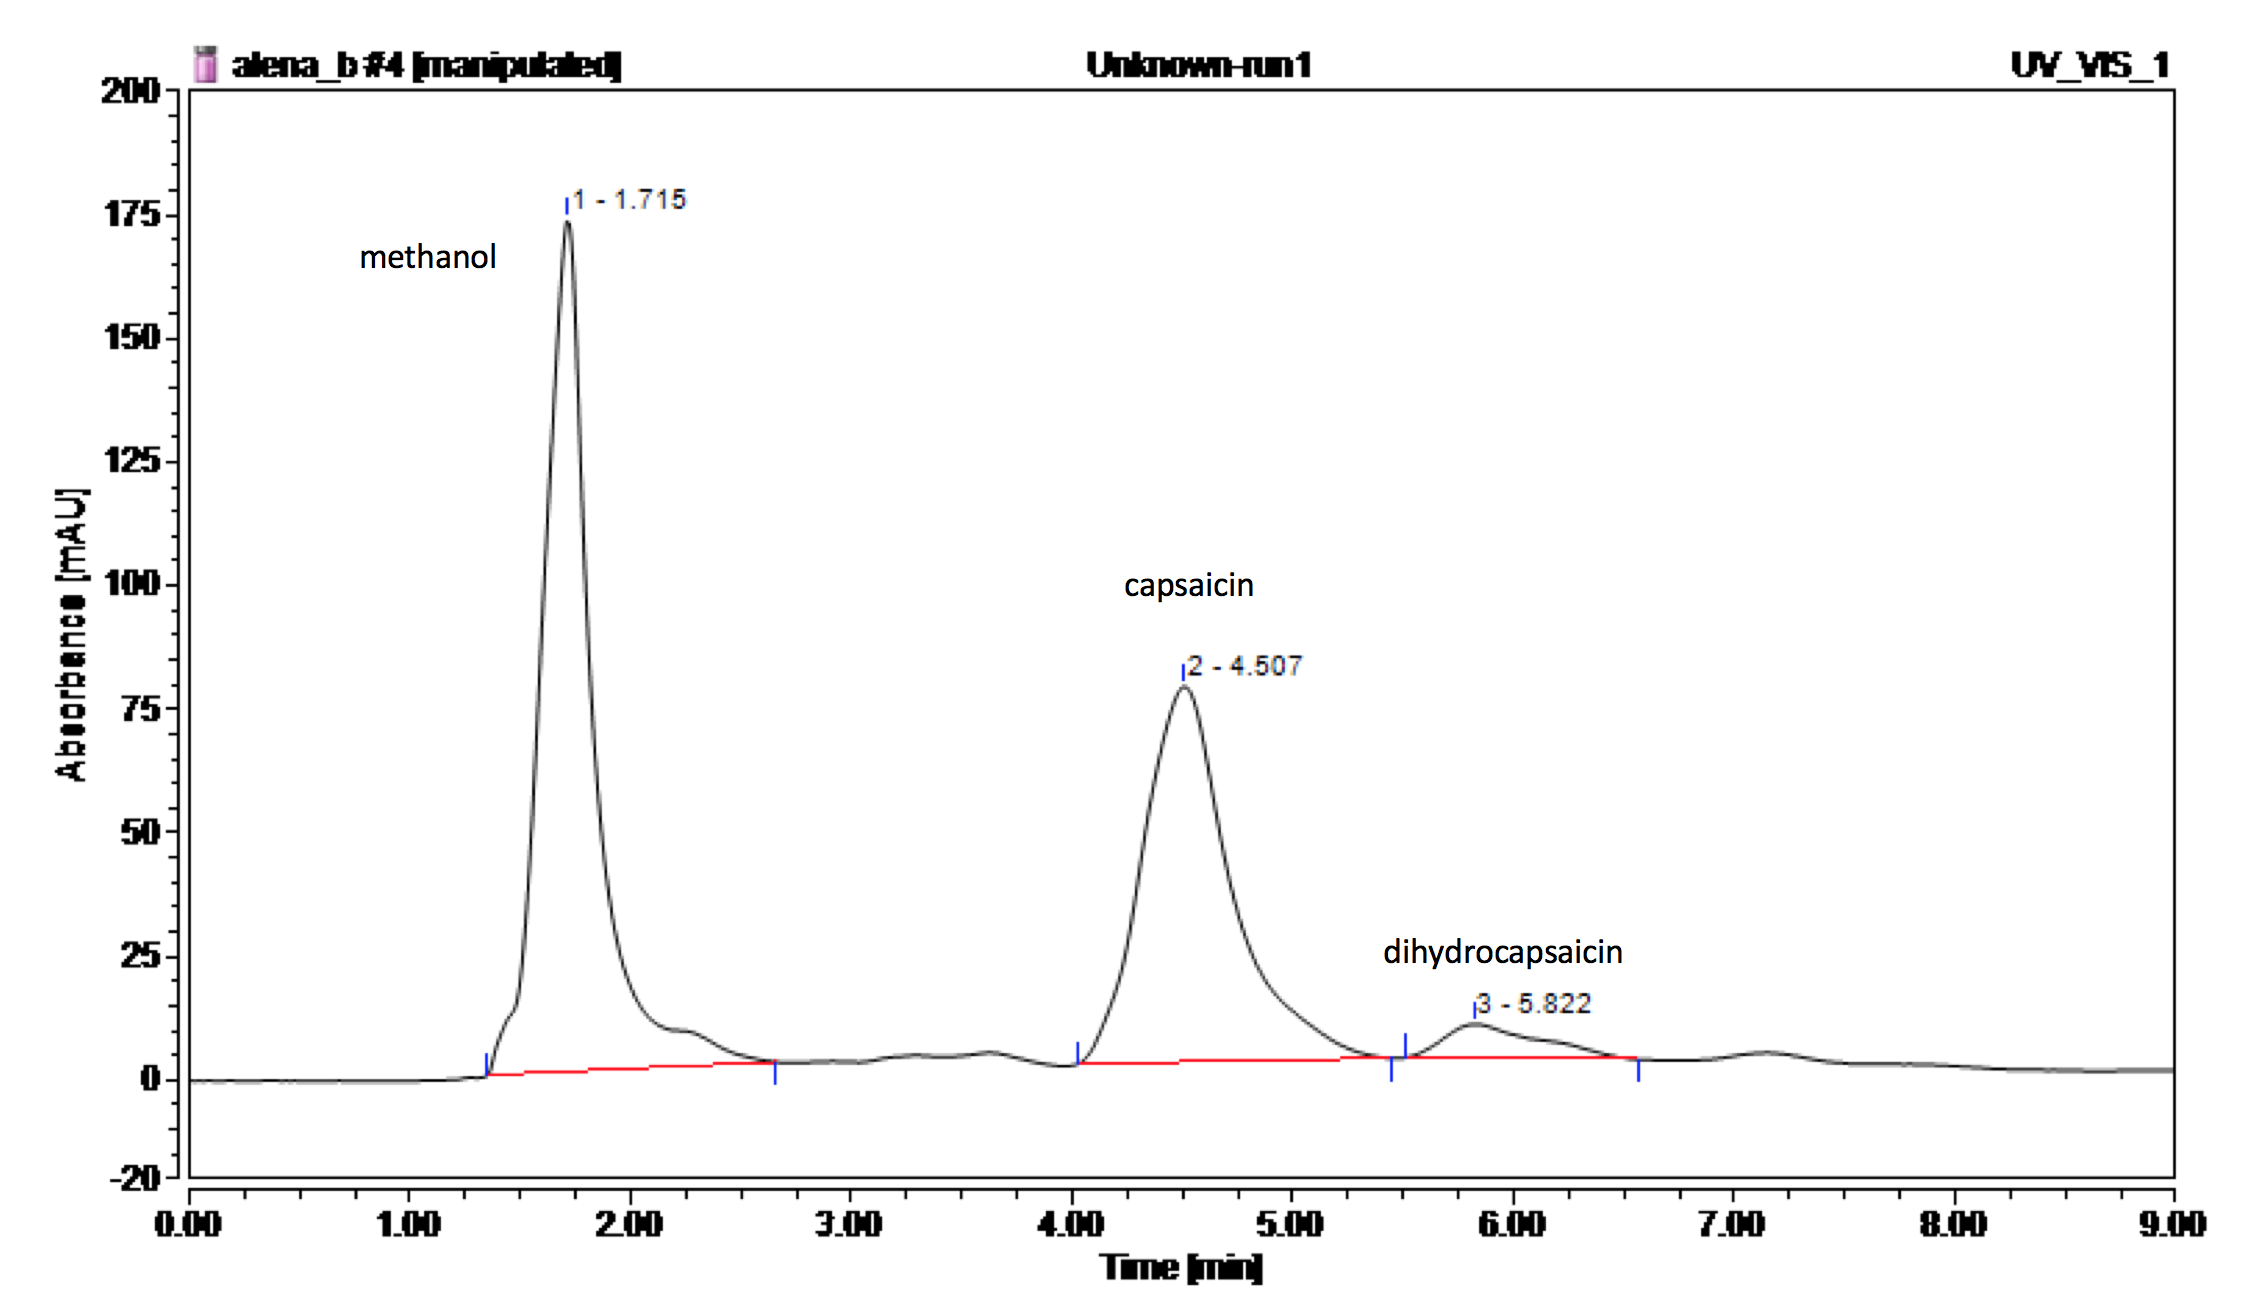
\includegraphics[scale=0.32]{unknown1}
    \captionof{figure}{Chromatogram of unknown solution, run 1.}

\vspace{5cm}
    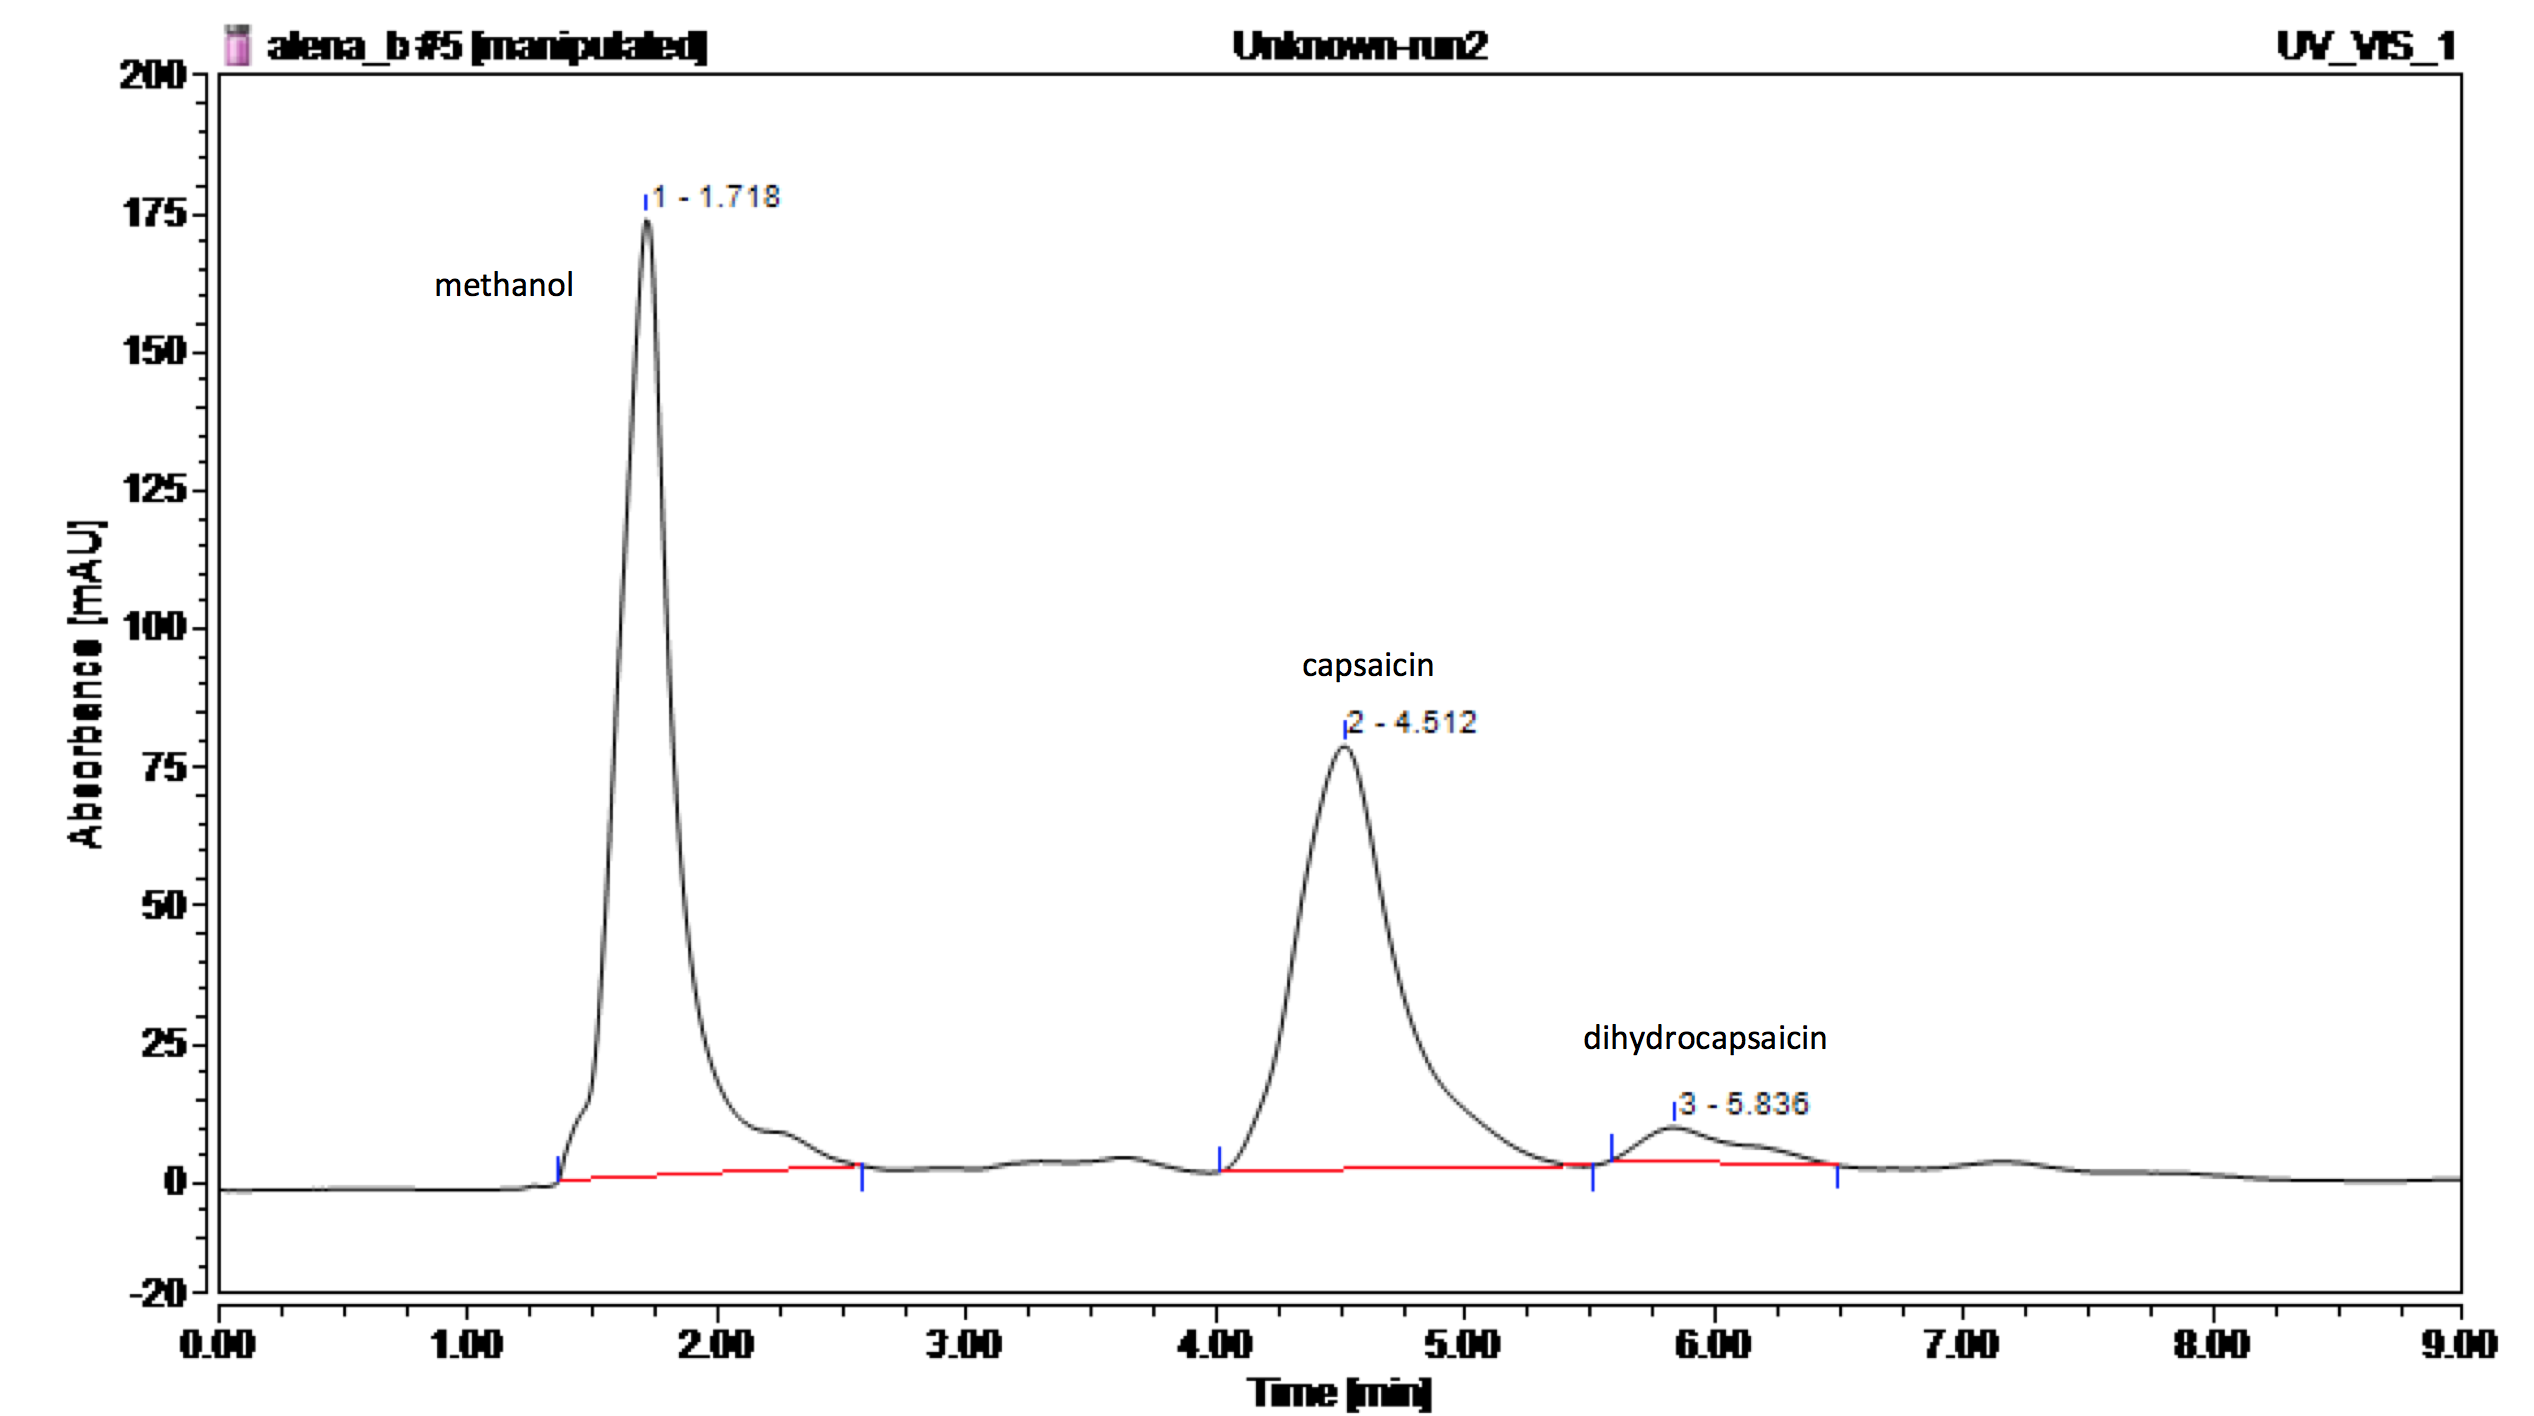
\includegraphics[scale=0.3]{unknown2}
    \captionof{figure}{Chromatogram of unknown solution, run 2.}

\vspace{5cm}
    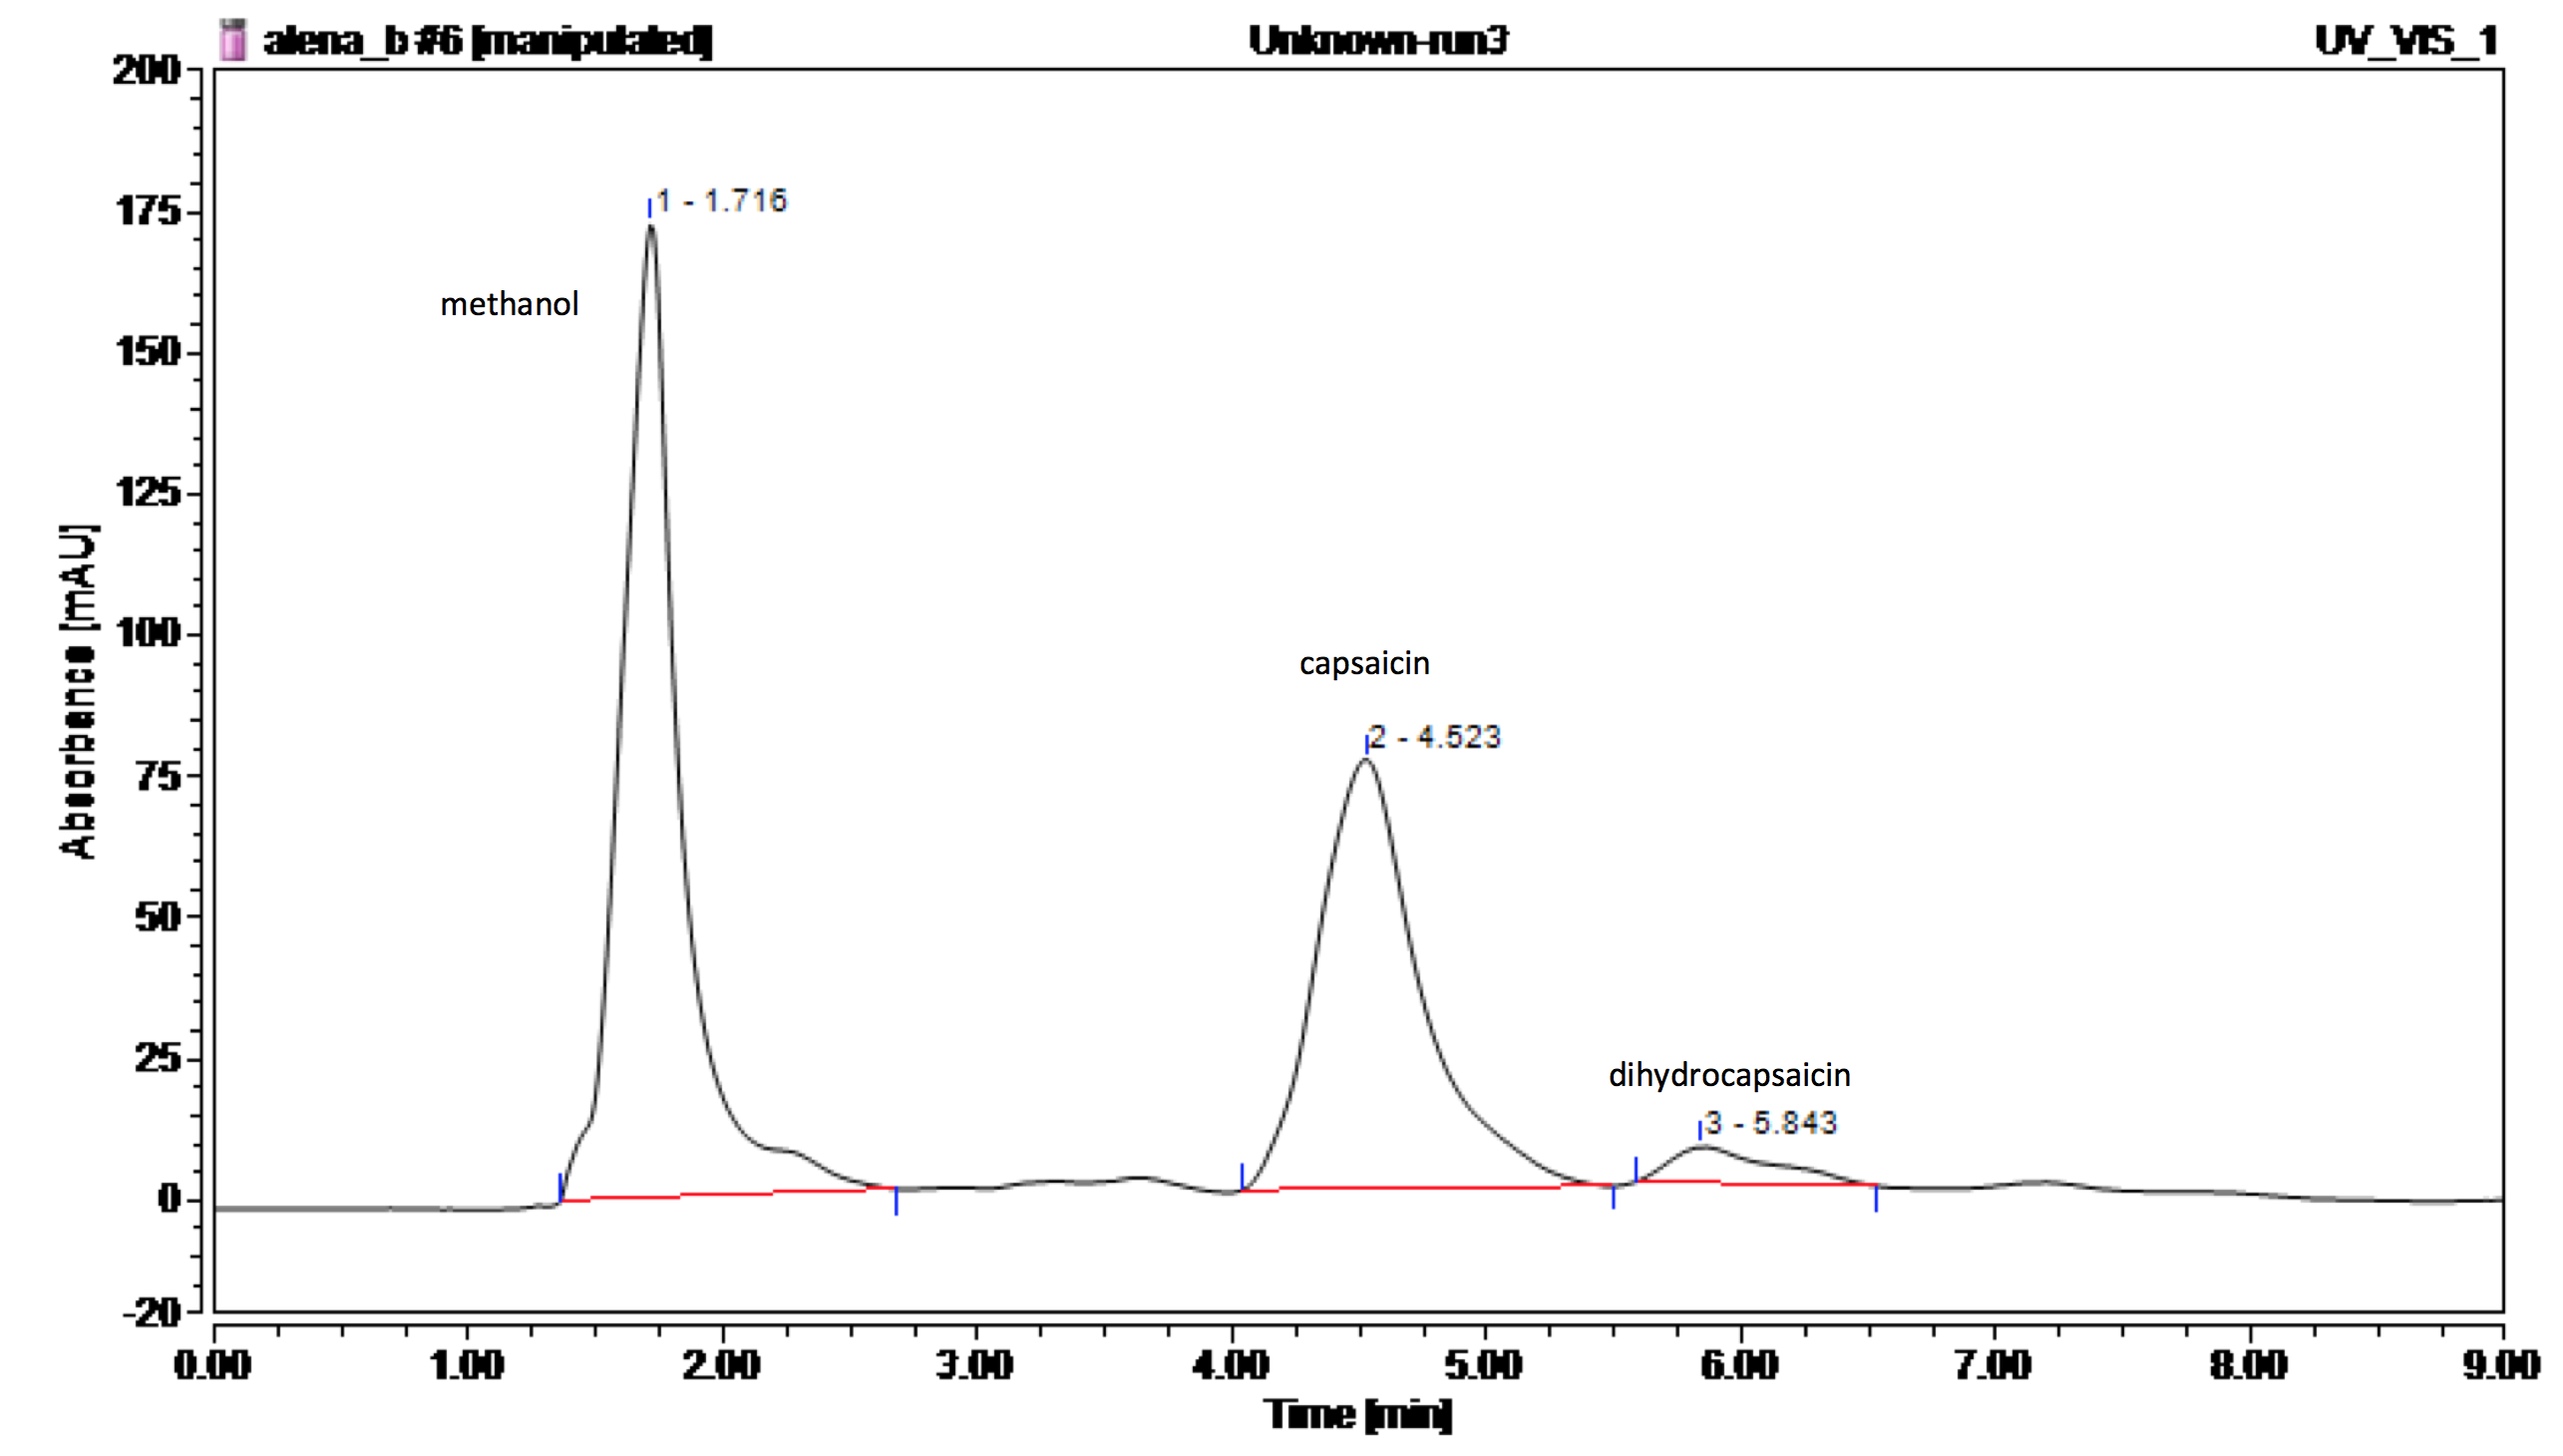
\includegraphics[scale=0.3]{unknown3}
    \captionof{figure}{Chromatogram of unknown solution, run 3.}

\vspace{5cm}
    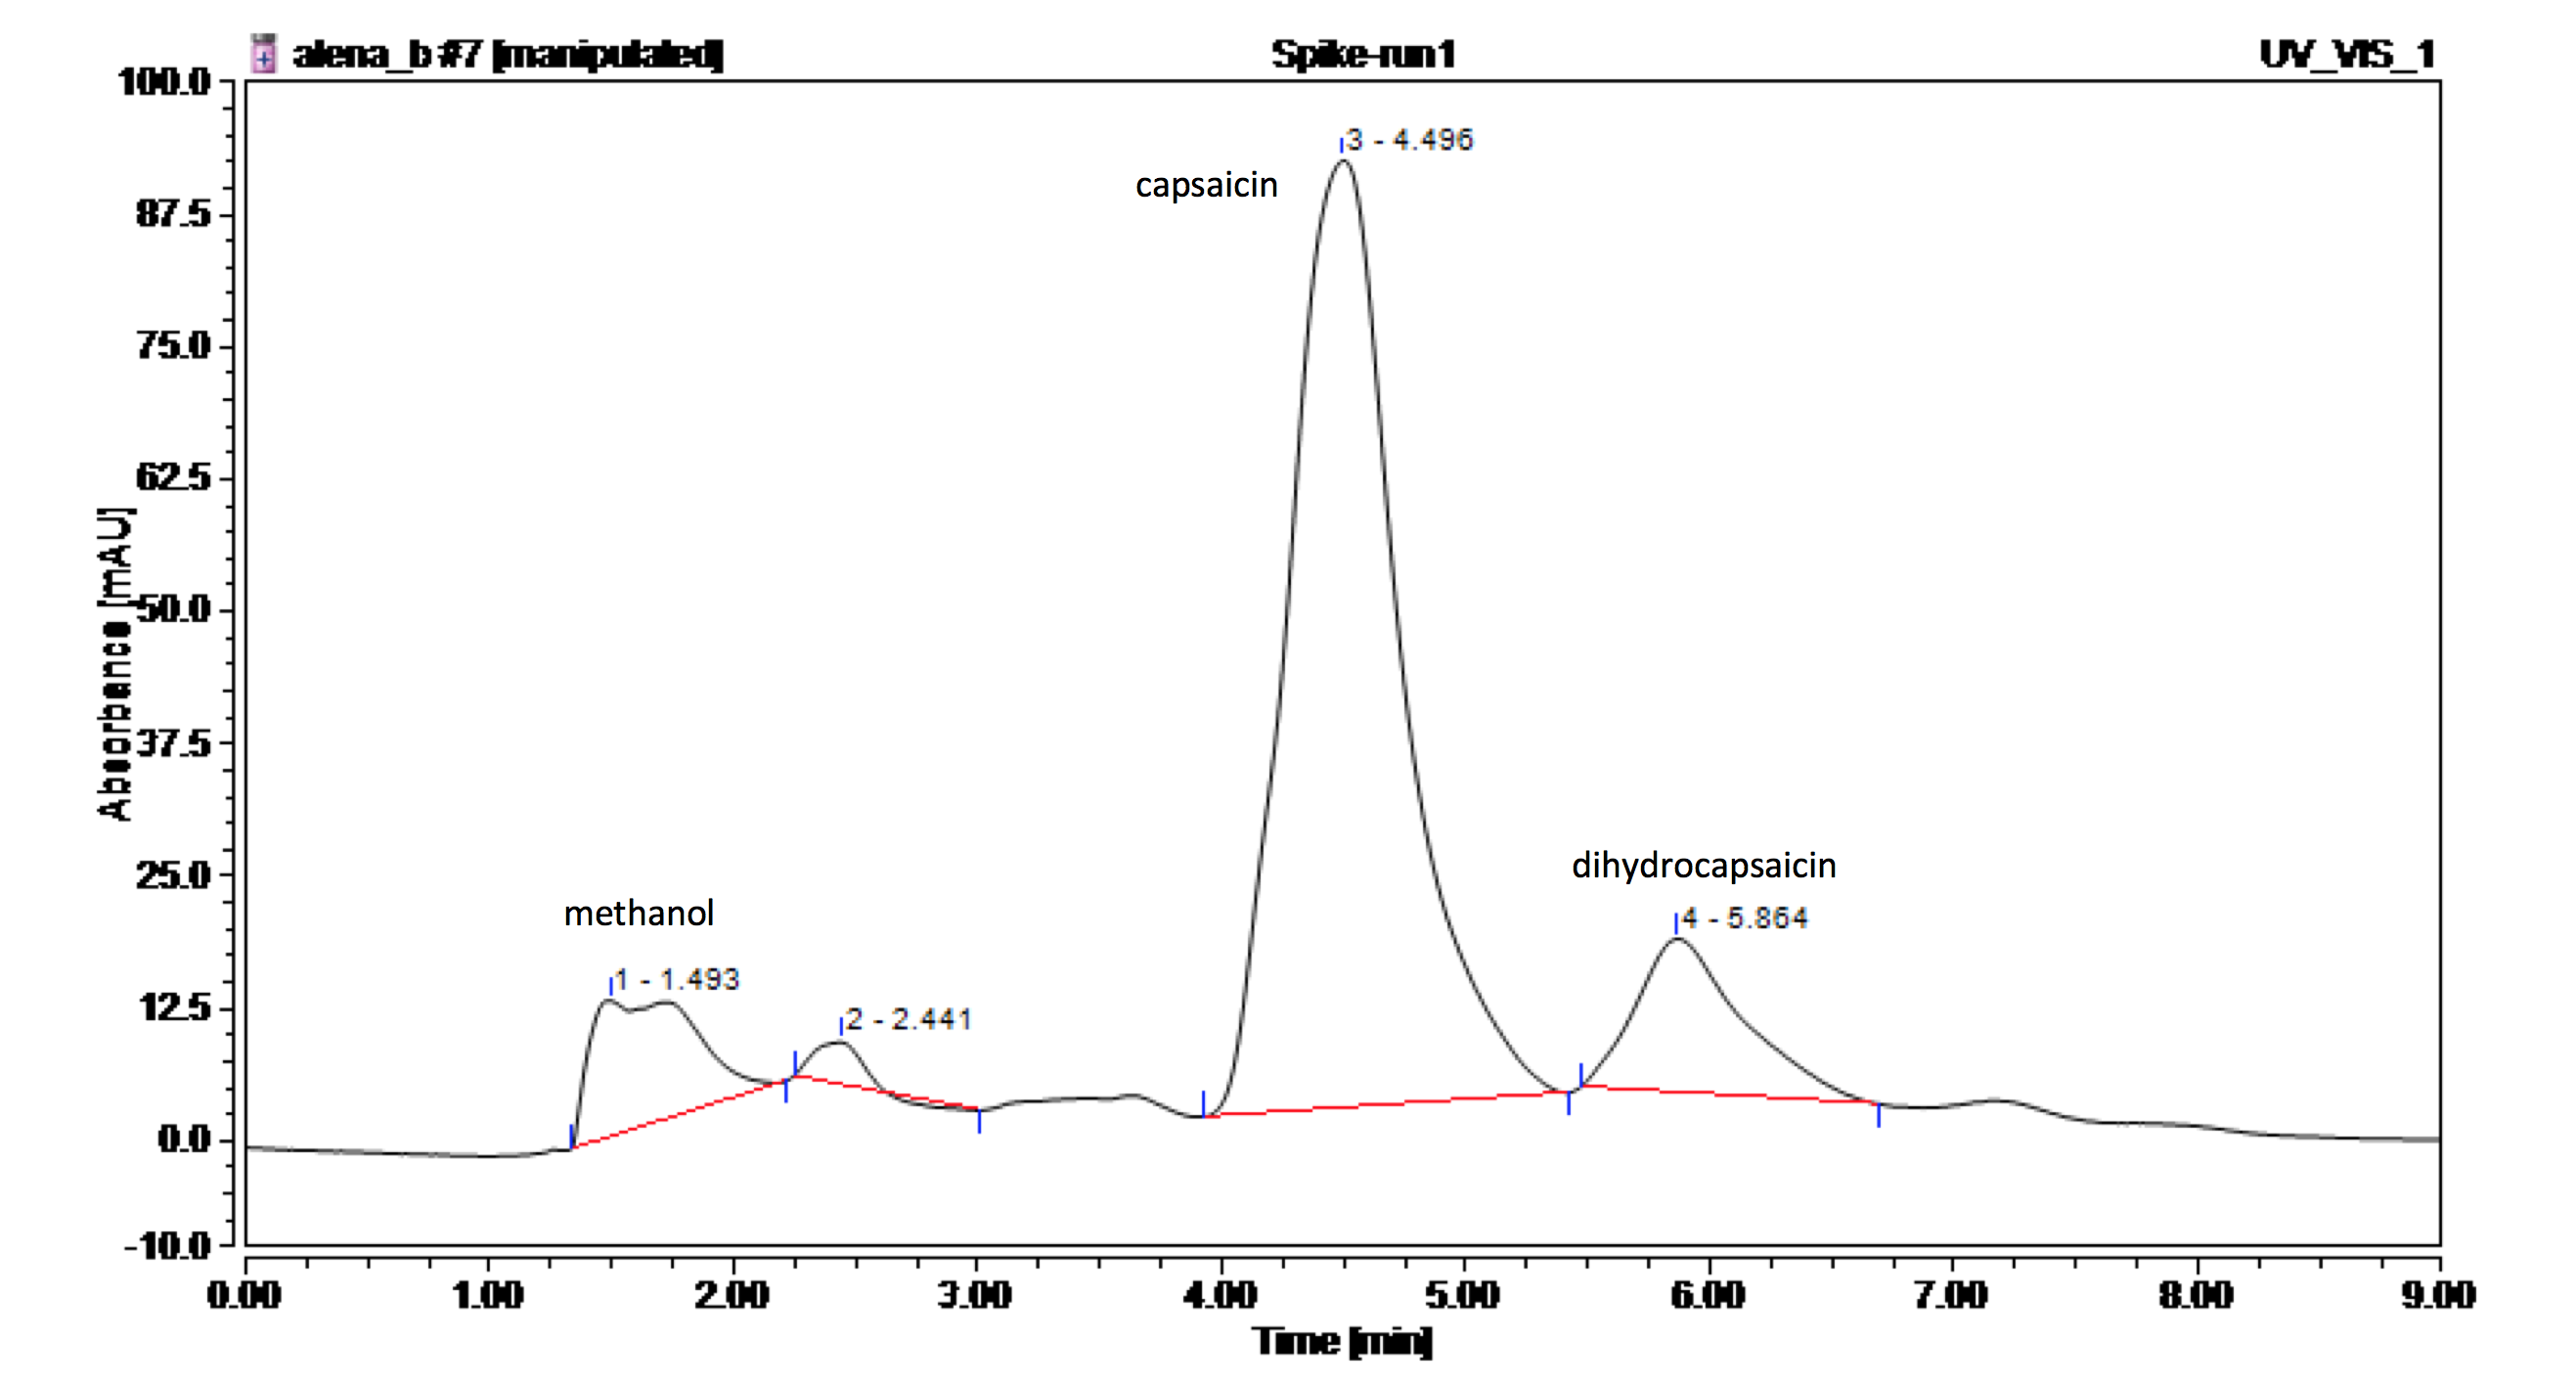
\includegraphics[scale=0.3]{spike1}
    \captionof{figure}{Chromatogram of spiked unknown solution, run 1.}

\vspace{5cm}
    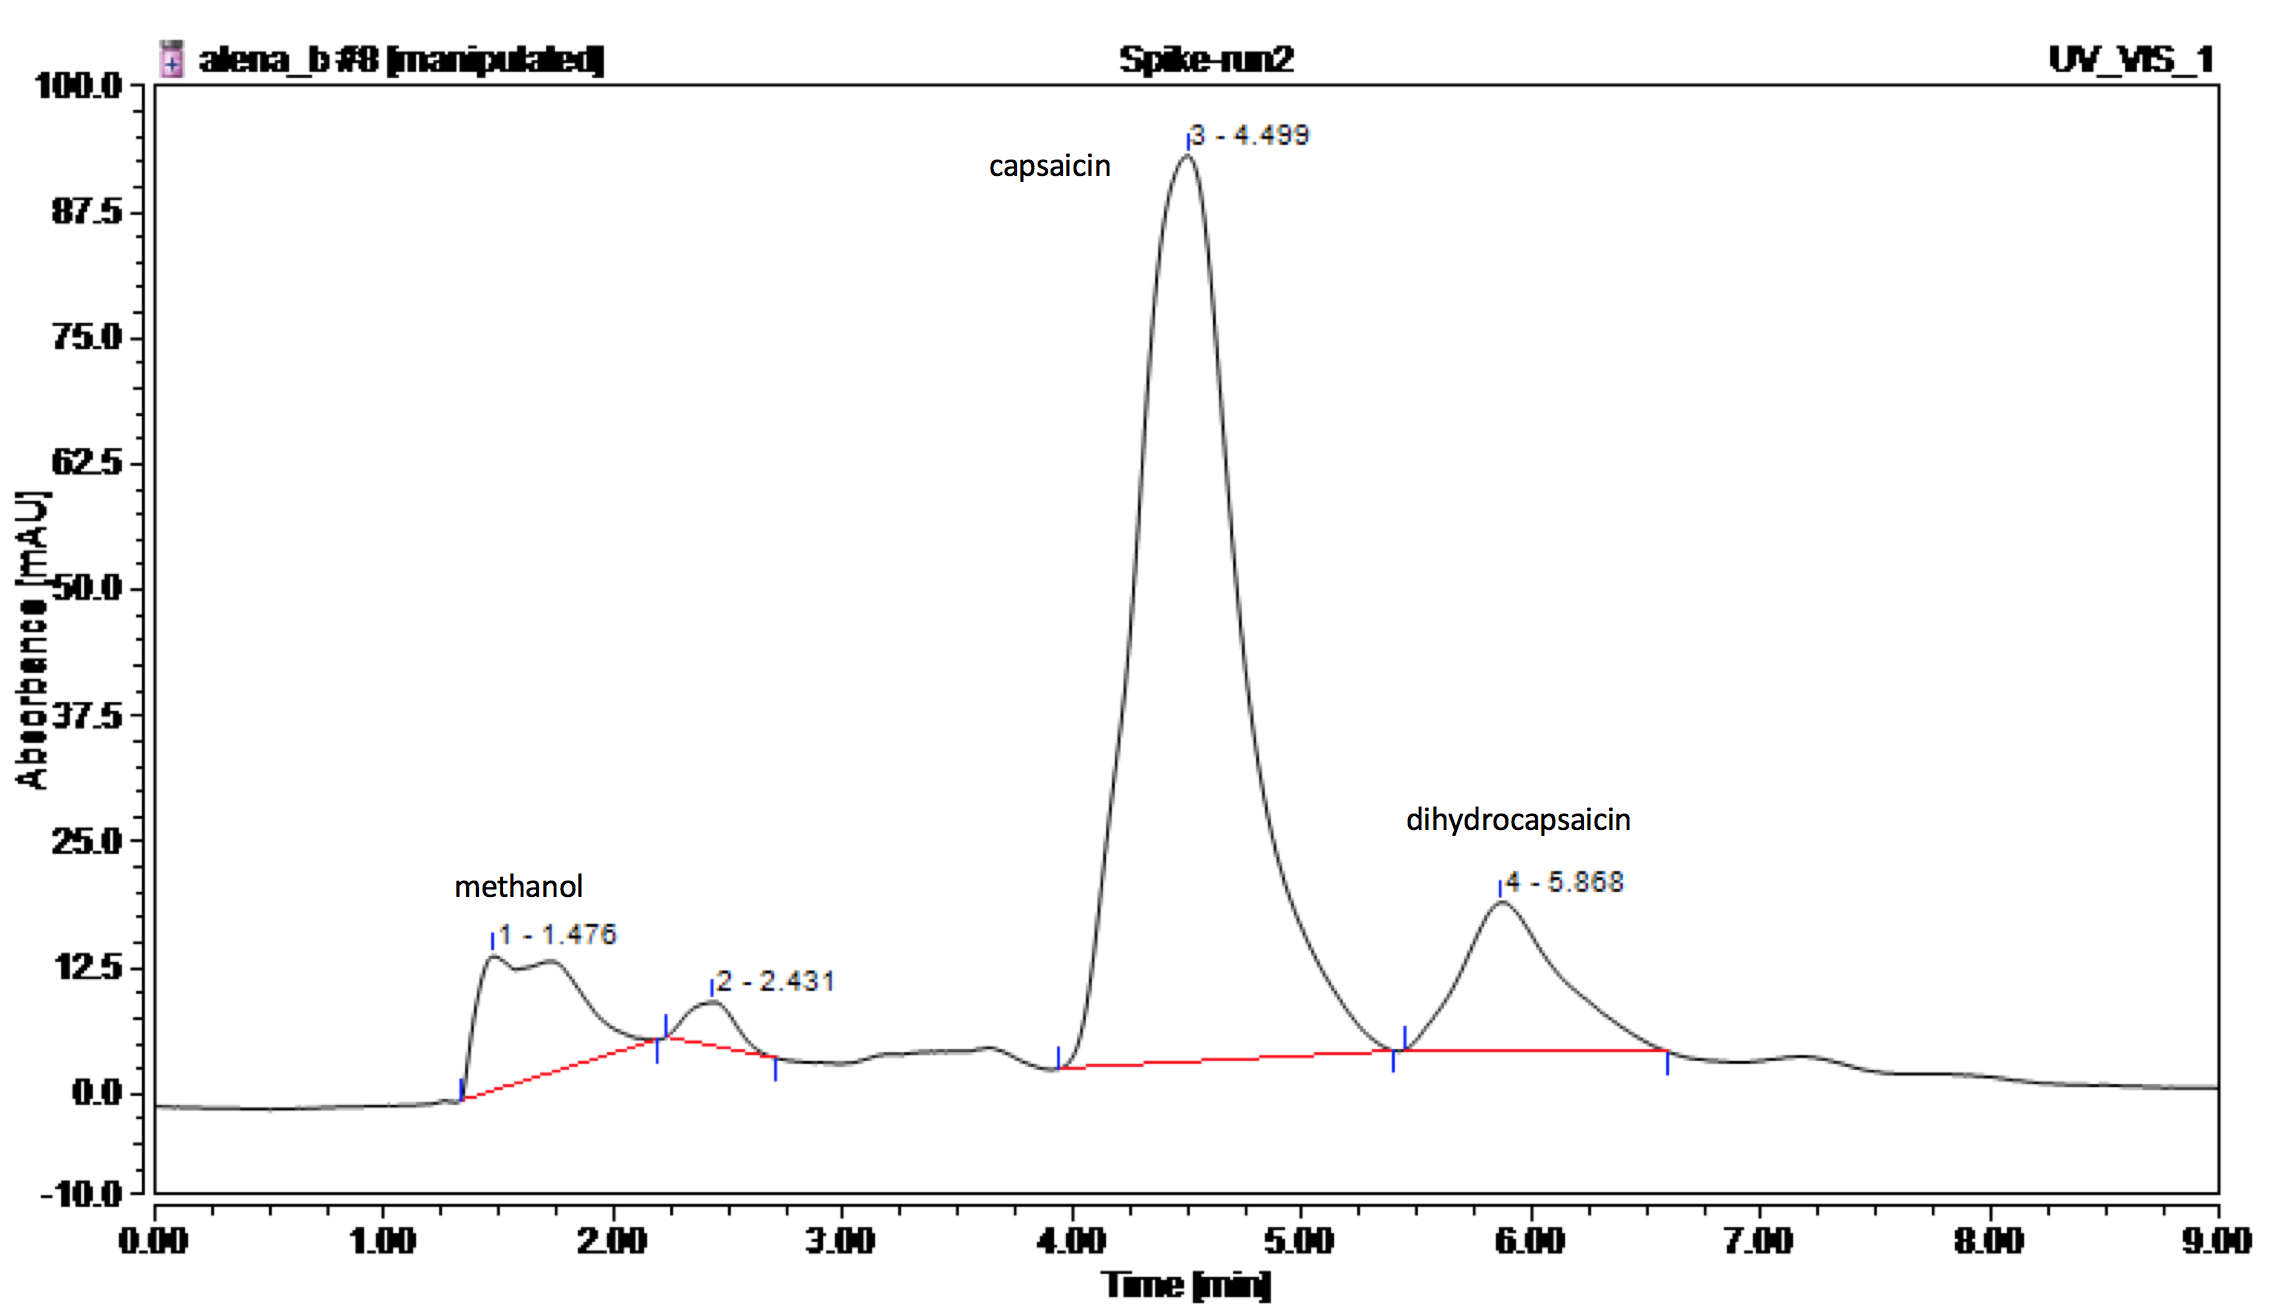
\includegraphics[scale=0.32]{spike2}
    \captionof{figure}{Chromatogram of spiked unknown solution, run 2.}

\vspace{5cm}
    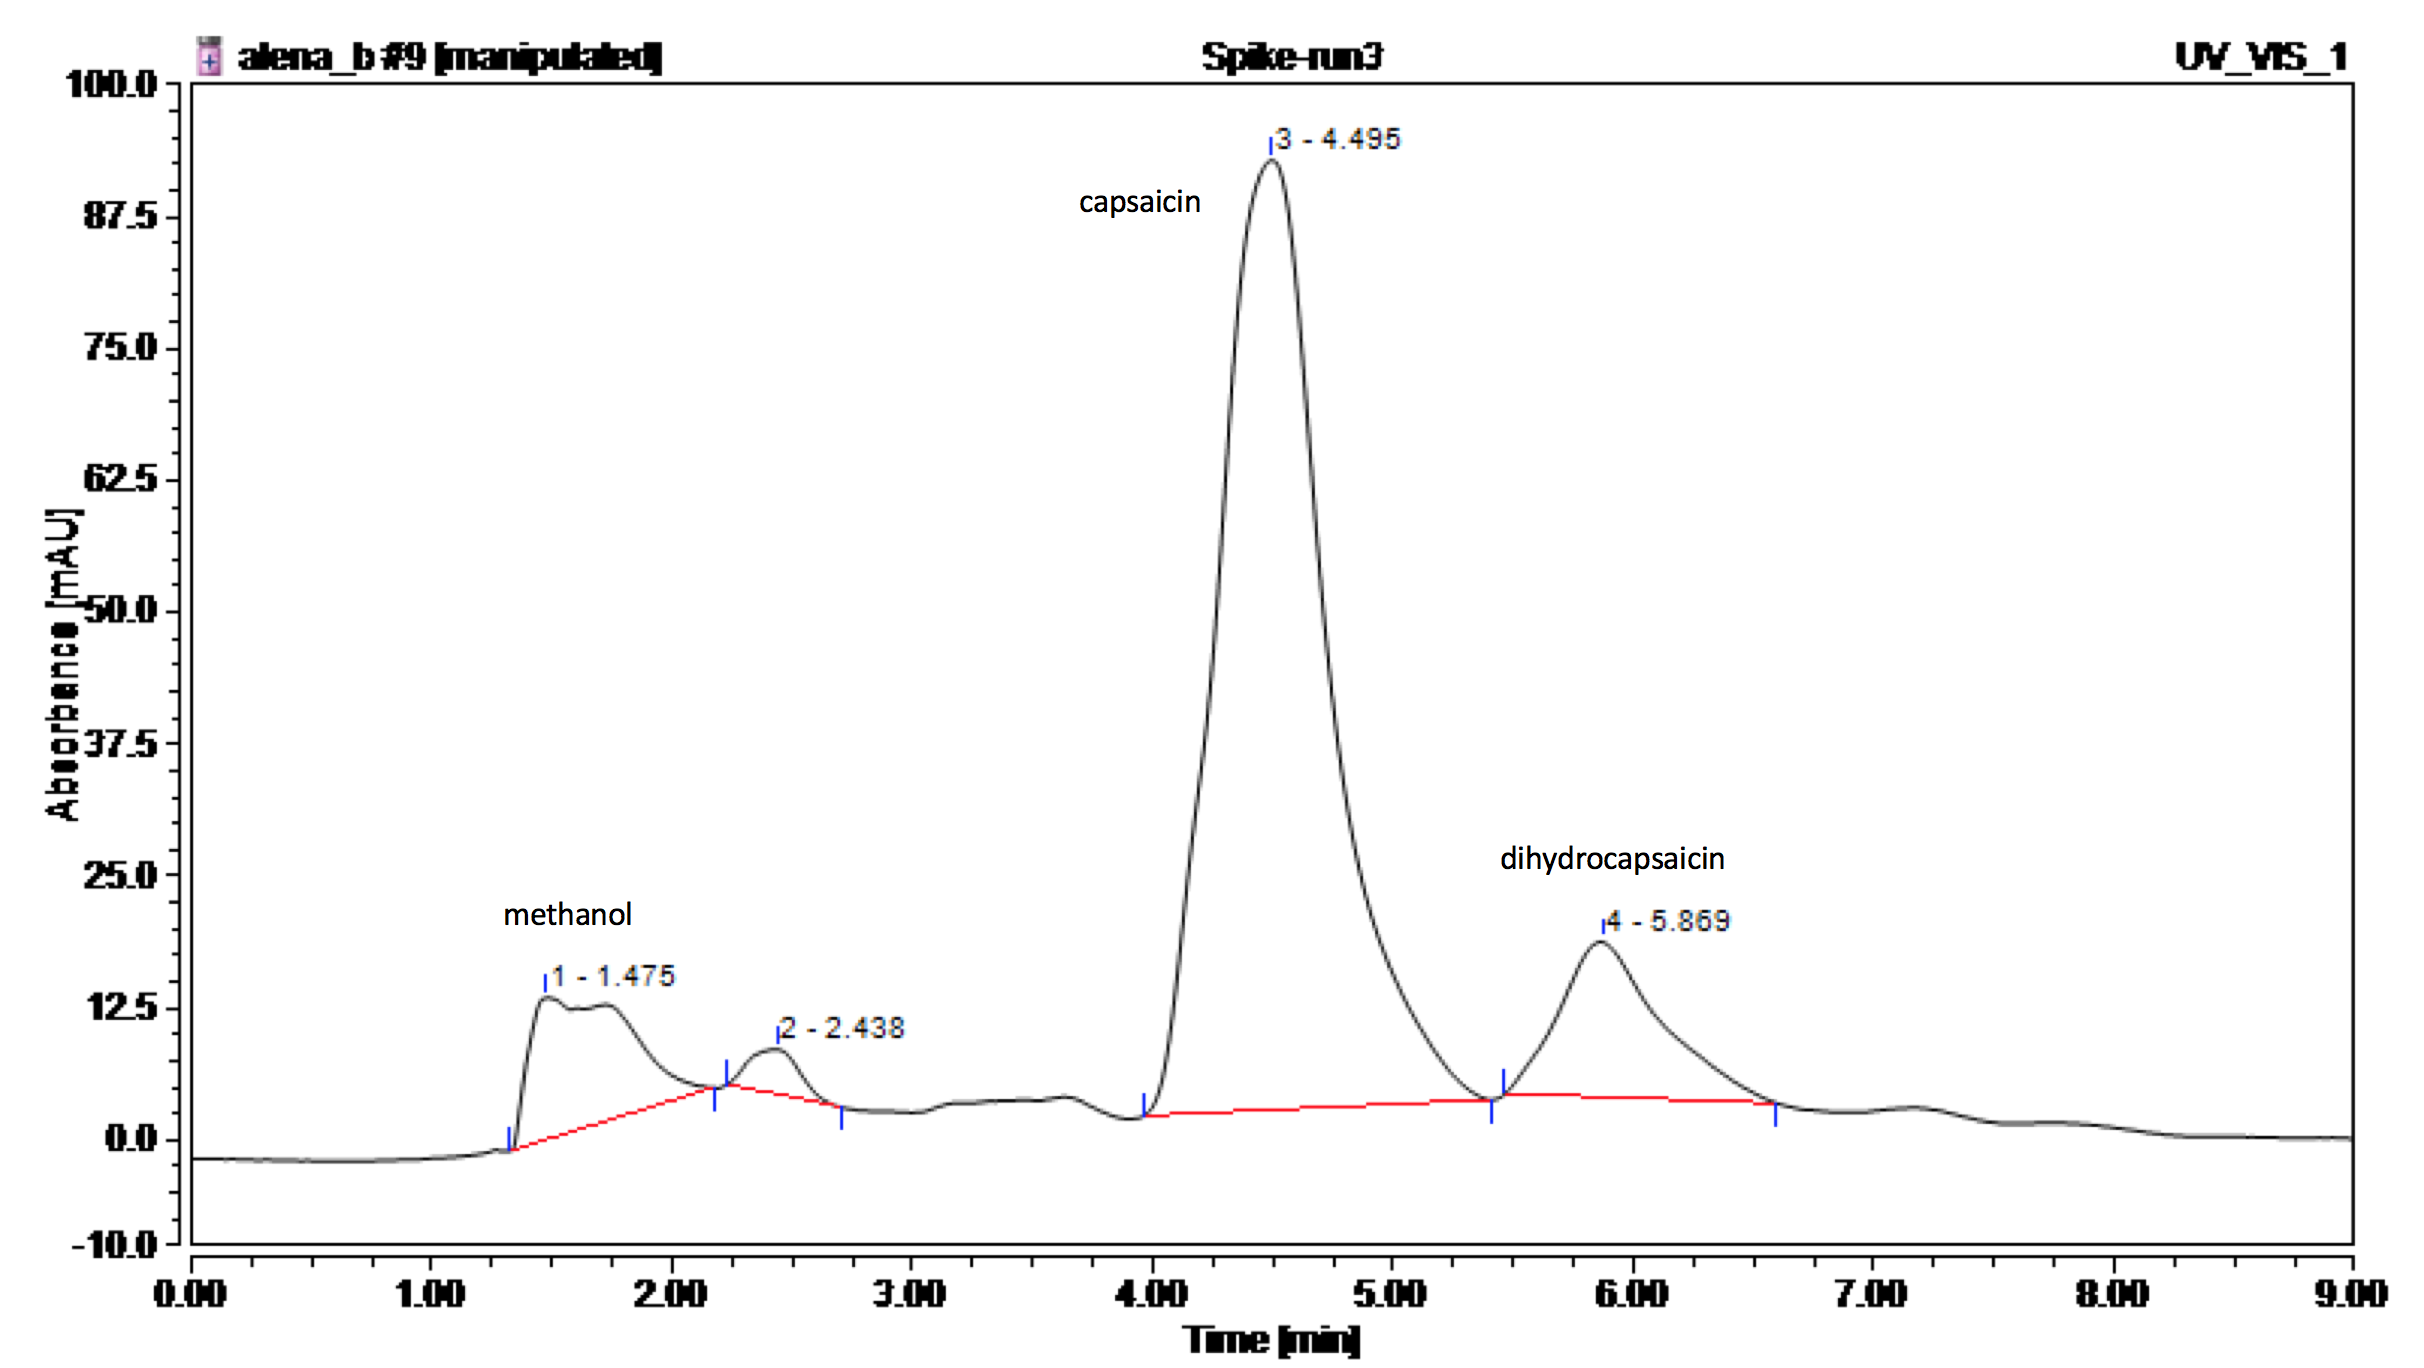
\includegraphics[scale=0.3]{spike3}
    \captionof{figure}{Chromatogram of spiked unknown solution, run 3.}

\newpage
	\captionof{table}{Analysis of Standard solutions.}
    \resizebox{0.7\textwidth}{!}{\begin{tabular}{lrrr}
    \textbf{Capsaicin} & \multicolumn{1}{l}{concentration (ppm)} & \multicolumn{1}{l}{retention time (min)} & \multicolumn{1}{l}{peak area (mAU*min)} \\
	\hline
    1 mL & 16.59 & 4.405 & 5.192 \\
    2 mL & 33.18 & 4.394 & 10.360 \\
    5 mL & 82.94 & 4.386 & 25.247 \\
	\\
    \textbf{Dihydrocapsaicin} & & & \\
	\hline
    1 mL & 8.932 & 5.860 & 1.978 \\
    2 mL & 17.86 & 5.851 & 3.568 \\
    5 mL & 44.66 & 5.839 & 10.065 \\
    \end{tabular}}

\vspace{2cm}
	\captionof{table}{Added amount of capsaicinoids in spiked unknown and percent recovery.}
    \resizebox{0.5\textwidth}{!}{\begin{tabular}{lrr}
    & \multicolumn{1}{l}{Capsaicin} & \multicolumn{1}{l}{Dihydrocapsaicin} \\
	\hline
    Amount added (mg) & 0.0948 & 0.01822 \\
    Percent Recovery & 100\% & 100\% \\
    \end{tabular}}

\vspace{2cm}
    \captionof{table}{Capsaicinoid concentrations in unknown as determined from
    calibration curve.}
    \resizebox{0.7\textwidth}{!}{\begin{tabular}{lrrrr}
    & \multicolumn{1}{l}{run1} & \multicolumn{1}{l}{run2} & \multicolumn{1}{l}{run3} & \multicolumn{1}{l}{average} \\
	\hline
    Capsaicin & 114.154093 & 115.390048 & 115.361156 & 115.0 \\
    Dihydrocapsaicin & 16.222512 & 13.7149066 & 14.371143 & 14.8 \\
    \end{tabular}}

\vspace{2cm}
    \captionof{table}{Capsaicinoid concentrations in spiked unknown as determined from
    calibration curve.}
    \resizebox{0.7\textwidth}{!}{\begin{tabular}{lrrrr}
    & \multicolumn{1}{l}{run1} & \multicolumn{1}{l}{run2} & \multicolumn{1}{l}{run3} & \multicolumn{1}{l}{average} \\
	\hline
    Capsaicin & 208.877879 & 210.624946 & 209.873099 & 209.8 \\
    Dihydrocapsaicin & 33.1673186 & 33.2629292 & 32.6327684 & 33.02 \\
    \end{tabular}}

\vspace{2cm}
	\captionof{table}{Peak areas of unknown (mAU$\times$min).}
    \resizebox{0.5\textwidth}{!}{\begin{tabular}{lrrrr}
    & \multicolumn{1}{l}{run1} & \multicolumn{1}{l}{run2} & \multicolumn{1}{l}{run3} & \multicolumn{1}{l}{average} \\
	\hline
    Capsaicin & 35.583 & 35.968 & 35.959 & 35.837 \\
    Dihydrocapsaicin & 3.457 & 2.88 & 3.031 & 3.12 \\
    \end{tabular}}
	
\vspace{2cm}
	\captionof{table}{Peak areas of spiked unknown (mAU$\times$min).}
    \resizebox{0.5\textwidth}{!}{\begin{tabular}{lrrrr}
    & \multicolumn{1}{l}{run1} & \multicolumn{1}{l}{run2} & \multicolumn{1}{l}{run3} & \multicolumn{1}{l}{average} \\
	\hline
    Capsaicin & 47.787 & 48.189 & 48.016 & 47.997 \\
    Dihydrocapsaicin & 7.356 & 7.378 & 7.233 & 7.322 \\
    \end{tabular}}

\vspace{2cm}
	\captionof{table}{Retention times of unknown (min).}
    \resizebox{0.5\textwidth}{!}{\begin{tabular}{lrrrr}
    & \multicolumn{1}{l}{run1} & \multicolumn{1}{l}{run2} & \multicolumn{1}{l}{run3} & \multicolumn{1}{l}{average} \\
	\hline
    Capsaicin & 4.507 & 4.512 & 4.523 & 4.514 \\
    Dihydrocapsaicin & 5.822 & 5.836 & 5.843 & 5.834 \\
    \end{tabular}}

\vspace{2cm}
	\captionof{table}{Peak widths at half height of unknown (min).}
	\resizebox{0.5\textwidth}{!}{\begin{tabular}{lrrrr}
    & \multicolumn{1}{l}{run1} & \multicolumn{1}{l}{run2} & \multicolumn{1}{l}{run3} & average \\
	\hline
    Capsaicin & 0.404 & 0.405 & 0.407 & 0.405 \\
    Dihydrocapsaicin & 0.515 & 0.483 & 0.473 & 0.490 \\
    \end{tabular}}

\vspace{2cm}
	\captionof{table}{Separation efficiency parameters.}
    \resizebox{0.6\textwidth}{!}{\begin{tabular}{lll}
    & Capsaicin & Dihydrocapsaicin \\
	\hline
    Number of Theoretical Plates (N) & 689 & 787 \\
    Height Equivalent to a Theoretical Plate & 0.218 mm & 0.191 mm \\
    \end{tabular}}
\newpage

\subsection*{ Sample calculations of determining heat rating of capsaicin in
unknown sample.}
\vspace{2cm}

    Capsaicin concentration in unknown as determined from calibration
    curve = 115.0 ppm \\
    mass of hot sauce sample = 8.7797 g \\

\begin{align*}
    \text{concentration in sample before dilution with H$_2$O} (2 mL) &= (115.0
    ppm) (10 mL) \\
    \text{concentration in sample before dilution with H$_2$O} &= 575.0 ppm \\
    \frac{\text{weight of capsaicin in original}}{25 mL} &= \frac{575.0 mg}{1L}
    \\
\end{align*}

weight of capsaicin in original = 0.01438 g
\begin{align*}
    \frac{0.01438g}{8.7797g} &= 0.164\% \text{ wt capsaicin.} \\
    0.00164 \times 16.1\times 10^6 &= 26404 \text{ Scoville Units.} \\
\end{align*}

\end{center}
\end{document} 
